% Template LaTeX document for CSSR4Africa Deliverables
% Adapted from documents prepared by EPFL for the RobotCub project
% and subsequently by the University of Skövde for the DREAM project
%
% DV 28/06/2023

\documentclass{CSSRforAfrica}

\usepackage[titletoc,title]{appendix}
\usepackage[colorlinks, urlcolor=blue, linkcolor=black, citecolor=black]{hyperref}
\usepackage{latexsym}
\usepackage{comment}
\usepackage{multirow}
\usepackage{subcaption}
\usepackage[breakable,skins,most]{tcolorbox} % Consolidated tcolorbox options
\usepackage{tabularx,colortbl}
\usepackage[tikz]{bclogo} % for boxes
\usepackage{ragged2e}
\usepackage{dirtree}
\usepackage{listings}
\usepackage{textcomp}
\usepackage{natbib}
\usepackage{url}
\usepackage{graphicx}
\usepackage{array}
\usepackage{longtable}
\usepackage{cleveref}
\usepackage{enumitem}
\usepackage{setspace}
\usepackage{float}
\usepackage{svg}

\crefformat{figure}{Figure~#2#1#3}
\crefformat{section}{Section~#2#1#3}

\lstset{upquote=true}
\renewcommand{\DTstyle}{\footnotesize\sffamily}

\newcommand{\blank}{~\\}
\newcommand{\checkbox}{{~~~~~~~\leavevmode \put(-7,-1.5){  \huge $\Box$  }}}


%%% for listing ; added by Pam %%%%%%%%%%%%%%%%%%%%%%%%%%%%%%
\captionsetup[figure]{format=hang}
\definecolor{codegreen}{rgb}{0,0.6,0}
\definecolor{codepurple}{rgb}{0.58,0,0.82} %% added by David Vernon from https://nasa.github.io/nasa-latex-docs/html/examples/listing.html
\definecolor{greenyellow}{rgb}{0.8, 0.7, 0.10}
\definecolor{backcolour}{rgb}{0.95,0.95,0.95} 

\lstdefinestyle{withoutNumbering}{
    backgroundcolor=\color{backcolour},   
    commentstyle=\color{codegreen},
    keywordstyle=\color{magenta},
    stringstyle=\color{codepurple},
    basicstyle=\ttfamily\small,
    breakatwhitespace=false,         
    breaklines=true,                 
    captionpos=b,                    
    keepspaces=true,                 
    showspaces=false,                
    showstringspaces=false,
    showtabs=false,                  
    tabsize=2
}

\begin{document}
\input{epsf}

%%
%% SHOULD NOT NEED TO BE CHANGED BEFORE THIS POINT
%% ------------------------------------------------
%%

\deliverable{D5.5.1.2}                   
\title{D5.5.1.2 Programming by Demonstration}     

\leadpartner{Carnegie Mellon University Africa}                       
\partner{}                                % INSERT partner name: Carnegie Mellon University Africa or The University of the Witwatersrand

\revision{1.3}                          
\deliverabledate{9/12/2024}   
\submissiondate{9/12/2024} 
\revisiondate{31/01/2025}                
\disseminationlevel{PU}
\responsible{Daniel Barros}           % REPLACE with correct  name


%%
%% Create the titlepage
%%

\maketitle
 

\section*{Executive Summary}
%===============================================================
\label{executive_summary}
%%\addcontentsline{toc}{section}{Executive Summary}
 
Deliverable 5.5.1.2 documents the development and functionality of a ROS package --- the PepperTrace Programming by Demonstration Tool --- designed to enable the Pepper robot to execute upper body and hand gestures learned through Programming by Demonstration (PbD). This software module is tailored for deployment on the real Pepper robot and is not intended for use in simulation.
\\~\\
\noindent
The deliverable includes the following.
\begin{itemize}
    \item The documented code for the \texttt{programming\_by\_demonstration} ROS package.
    \item A comprehensive report detailing the system architecture, component requirements, development procedures, and an explicit definition of the module's functional characteristics.
    \item Instructions for developers who wish to adapt the package for custom applications.
    \item A user manual to assist users in configuring and launching the module.
\end{itemize}
\noindent
The package's interface design covers input, output, and control data, while also specifying appropriate data structures. All development activities adhere to the software engineering standards outlined in Deliverable D3.2.
\\~\\
\noindent
%%Appendix I contains a user manual for the PepperTrace Programming by Demonstration tool.

\newpage
 
 
%\graphicspath{{./figs/}}
\pagebreak
\tableofcontents
\newpage


\section{Introduction}
%===============================================================
\hspace{0.5cm}This deliverable extends D5.5.1.1 Gesture Execution by introducing programming gestures by demonstration. This technique enables the robot to learn iconic and symbolic gestures directly from human demonstrators. Users interact with the system by performing gestures in front of an RGBD camera. Human joint positions are estimated using a skeletal model and retargeted to Pepper's joint angles. Various filters can be applied to increase the smoothness of imitation of the demonstrated movements.

The package includes a component for recording data from multiple Pepper sensors during the demonstration process. Additionally, a graphical user interface is provided to facilitate the control and management of demonstrations and data collection.

Section 2 specifies the requirements for the software module, covering functionality, performance, and usability aspects. Section 3 outlines the functional characteristics of the module, focusing on the retargeting of angles from the skeletal model to Pepper's joints. Section 4 addresses the interface design, specifying the data inputs, outputs, and control mechanisms. It also describes how these data are accessed or made available, whether through files or ROS mechanisms like subscribers, services, or actions. Section 5 details the module design, including implementation specifics and the connections between components. Section 6 provides instructions for running the PbD system. Section 7 documents the unit testing procedures for the module's components, ensuring reliability and performance. Finally, Section 8 offers guidance for developers on extending the software for custom applications.

\vspace{0.1cm}
\begin{figure}[ht!]
    \centering
    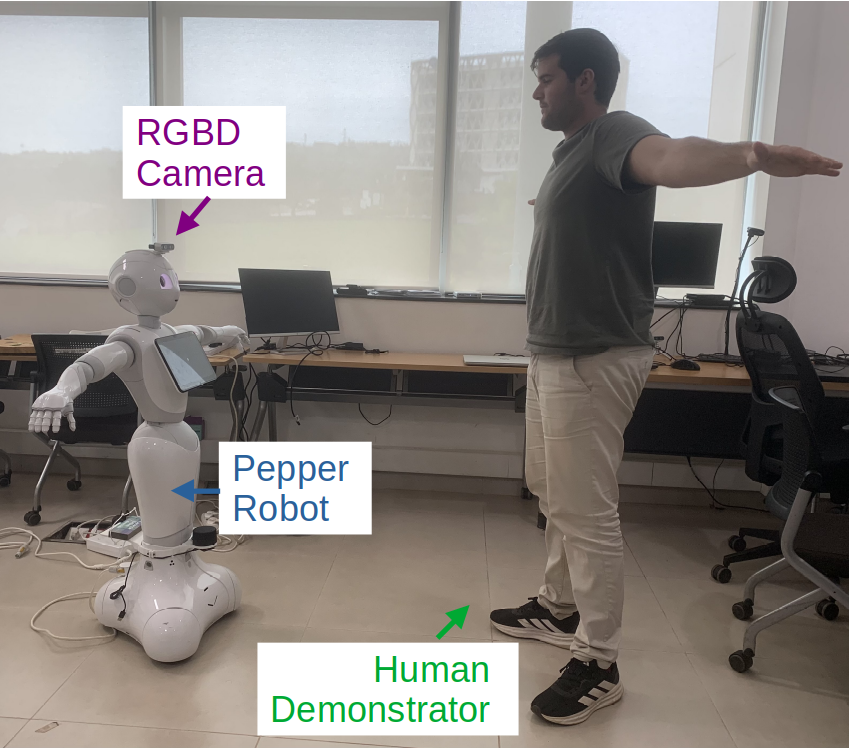
\includegraphics[width=13cm]{figures/setupPepper.png}
    \captionsetup{width=13cm}
    \caption{Programming by Demonstration Setup: The human demonstrator gestures in front of an RGBD camera and Pepper imitates the movements. }
    \label{fig:setup}
\end{figure}


 \newpage

\section{Requirements Definition}
%===============================================================
\begin{itemize}
    \item \textbf{Core Functionality:}
    \begin{itemize}
        \item The software must enable the Pepper robot to imitate upper-body gestures performed by humans in real-time (online) and from video (offline).
        \item Pepper should be able to imitate all gestures performed in the coronal plane and in front of the body.
        \item If joint angles cannot be calculated, the controller must maintain its previously commanded joint positions.
    \end{itemize}
    
    \item \textbf{Data Processing and Filtering:}
    \begin{itemize}
        \item A filtering function must smooth noisy angle estimations from the skeletal model, enhancing the naturalness of Pepper's movements.
        \item Switching between different filtering options should be easy and intuitive for the user.
    \end{itemize}
    
    \item \textbf{Demonstration and Recording:}
    \begin{itemize}
        \item The module must allow users to record demonstrations, storing data in an organized and accessible format.
        \item Recorded trajectories must be easy to store and replay.
        \item It should be possible to record any type of data coming from Pepper's sensors.
        \item The recording component must be expandable to support other user input modalities and robots.
    \end{itemize}
    
    \item \textbf{User Interface:}
    \begin{itemize}
        \item An intuitive user interface must be provided to facilitate control of the demonstration and recording process.
        \item Users must have real-time access to system logs during the demonstration process to gain operational insights.
    \end{itemize}
\end{itemize}


\newpage

\section{Module Specification}
The Programming by Demonstration module, also referred to as PepperTrace module, consists of three components. The first one, \texttt{skeletal\_model}, addresses the first and second set of requirements by enabling Pepper to imitate the upper body movements of a human demonstrator. The second one, \texttt{demonstration\_recorder}, deals with the third set of requirements by implementing data collection from the Pepper robot. Finally, the \texttt{demonstration\_gui} delivers an intuitive graphical user interface. \cref{fig:functionalgraph} provides the functional graph as the system overview.


\begin{figure}[ht!]
    \centering
    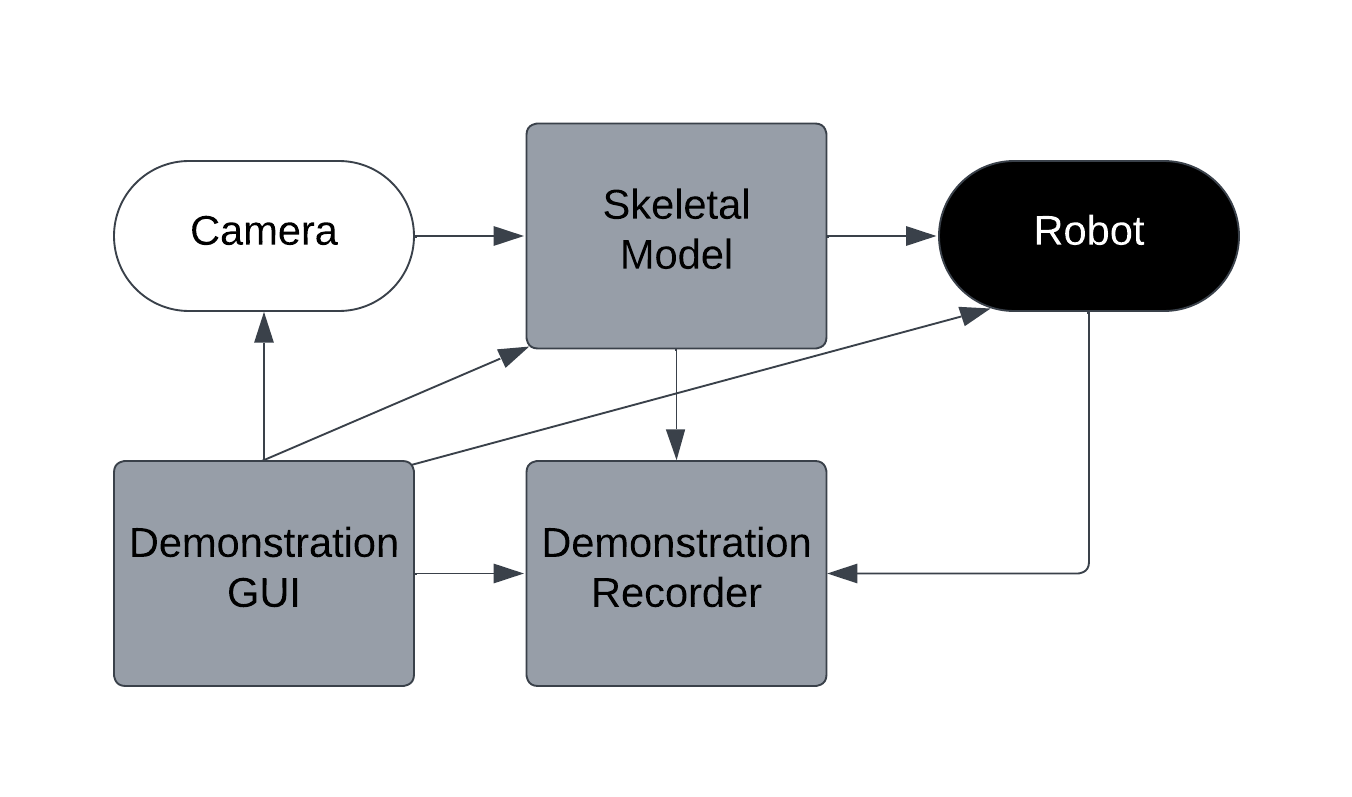
\includegraphics[width=0.8\textwidth]{figures/FunctionalGraph.png}
    \captionsetup{width=0.8\textwidth}
    \caption{Functional graph of the PbD module: the Skeletal Model processes visual and depth images to generate joint commands for the robot; the Demonstration Recorder logs these commands and data from the robot sensors; the Demonstration GUI provides user control over all the other components. The camera can be replaced by a pre-recorded video feed. }
    \label{fig:functionalgraph}
\end{figure}

\vspace{0.5cm}
The main computation is carried out in the \texttt{skeletal\_model} component, as shown in \cref{fig:computationalgraph}. By retargeting human joint positions to humanoid joint angles, the Pepper robot is endowed with the ability to imitate upper-body gestures performed by the human demonstrator. Occlusions of arm joints are not handled, so only movements in the coronal plane and in front of the body are imitated. As soon as one landmark on the human upper body is not detected in the frame, no new command will be sent, and Pepper's arm controllers will maintain the last commanded joint angles.

The input to this component is abstracted as visual and depth images, meaning the source incoming frames can be either a live image feed or a prerecorded video stream. This component also includes filtering of the retargeted joint angles to smooth noisy angle estimations from the skeletal model, enhancing the naturalness of Pepper’s movements.


\newpage

\begin{figure}[ht!]
    \centering
    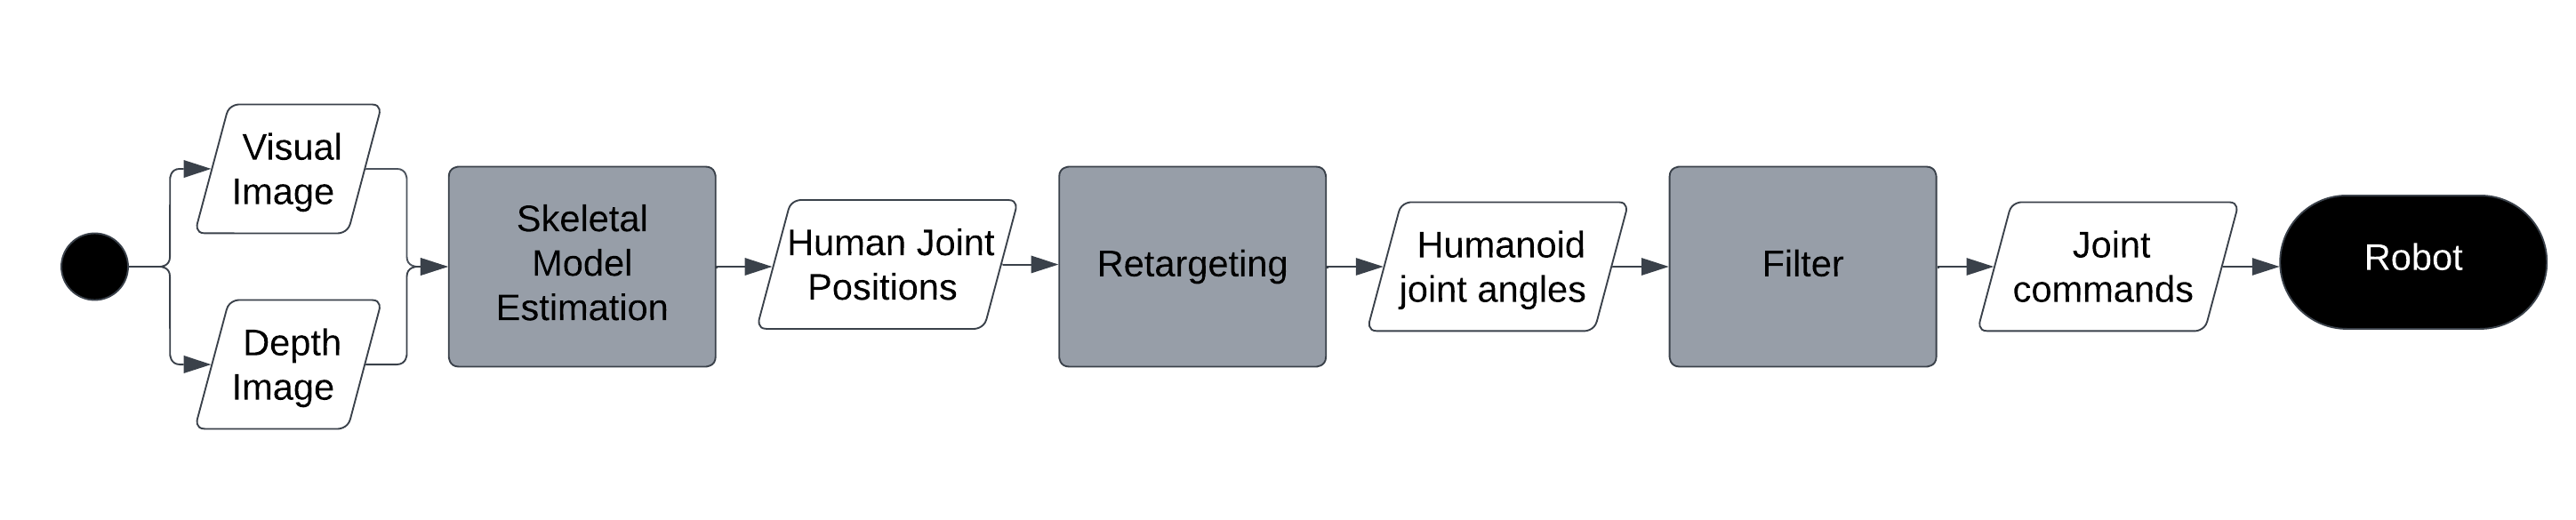
\includegraphics[width=\textwidth]{figures/ComputationalGraph.png}
    \captionsetup{width=\textwidth}
    \caption{Computational graph of the PbD module: Synchronized visual and depth images from the camera are used to estimate the skeletal model, i.e. the positions of the human joints. These are then retargeted to the joint angles of the Pepper humanoid robot. A filter is applied to the incoming joint angles to increase the naturalness of the movement in real-time and the resulting joint commands are fed to the robot arm controllers.  }
    \label{fig:computationalgraph}
\end{figure}  

The \texttt{demonstration\_recorder} component can be seen as the backend of the application. It provides a robust recording function that saves data locally in a consistent, structured format. This recorded data can be replayed by the robot, as illustrated in \cref{fig:statemachinegraph} and \cref{fig:behaviouralgraph}. The component integrates with the GUI to handle user inputs and display system information, offering an intuitive interface for users.

Designed with a modular approach, the \texttt{demonstration\_recorder} component can be customized for various robot platforms and user input devices. While the default user interface is the GUI provided by the \texttt{demonstration\_gui} component, developers have the flexibility to integrate alternative or additional input methods (see \cref{sec:anotherinput} for details).


\begin{figure}[H]
    \centering
    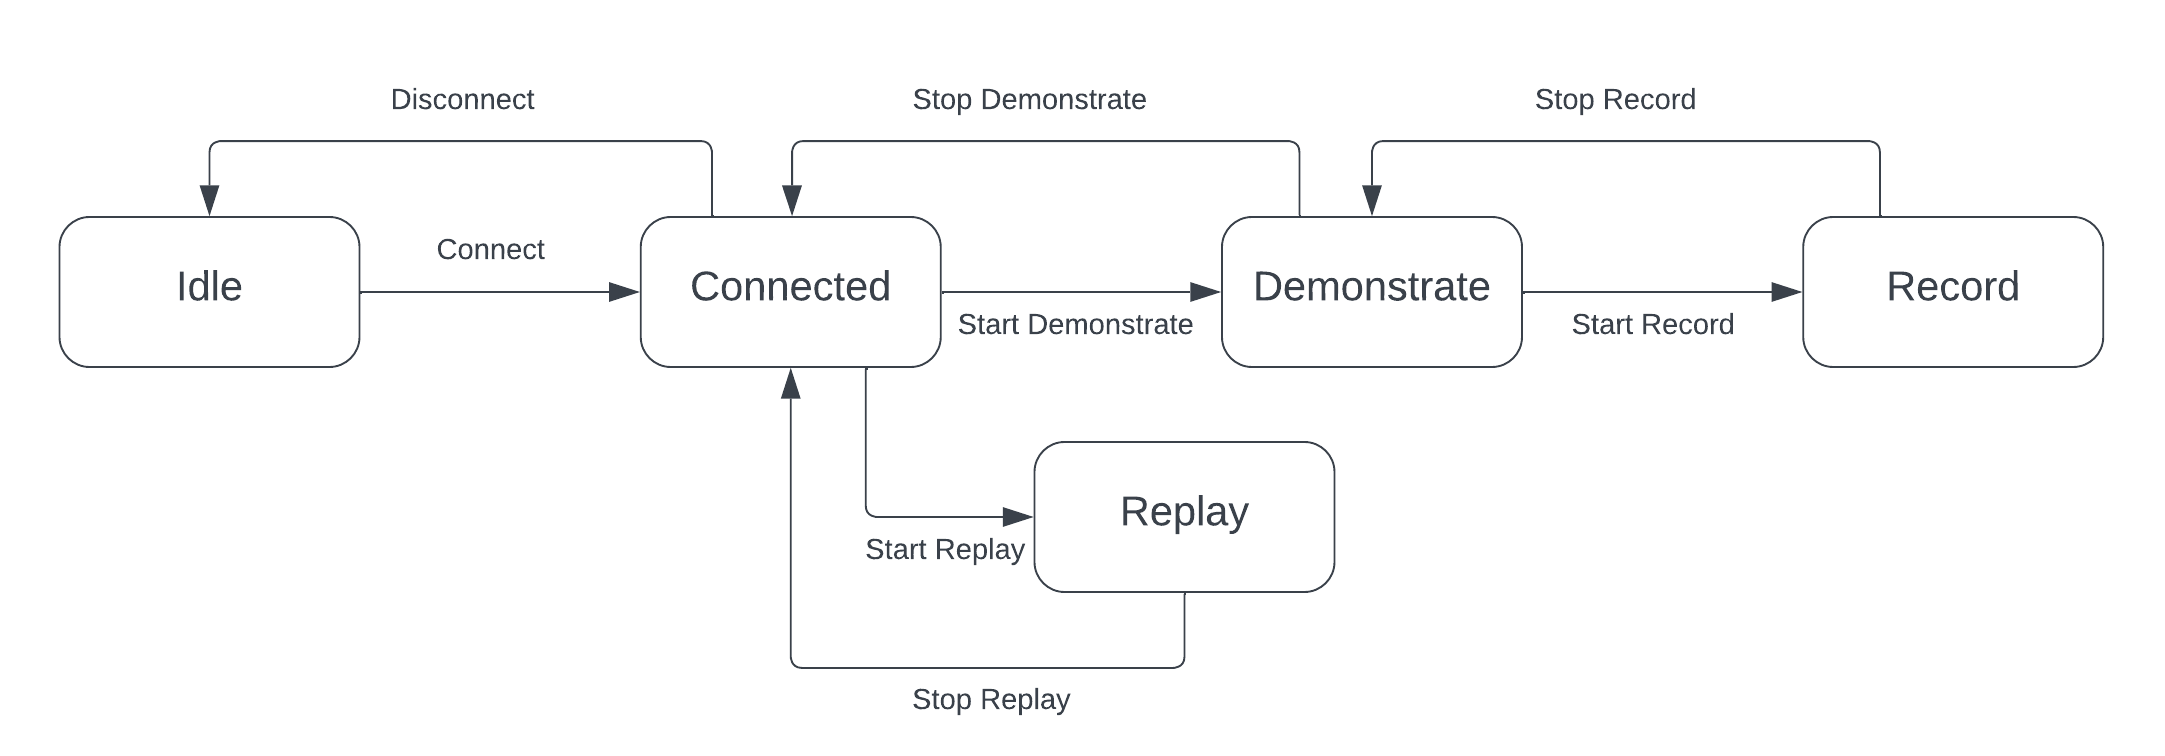
\includegraphics[width=\textwidth]{figures/StateMachineGraph.png}
    \captionsetup{width=\textwidth}
    \caption{State machine graph of the PbD module: Barring internal errors that are displayed to the user in the terminal and the GUI, binary user input determines the state of the system: every active state has an entry and exit function that needs to be explicitly called. Exception is ``Stop Replay", which can be stopped manually or stops automatically when the recorded motion has been fully performed. }
    \label{fig:statemachinegraph}
\end{figure}  
\newpage 
The GUI serves as the frontend for controlling the system’s functionality. It allows users to initiate and manage recordings, configure the types of data to be recorded, and select filters to apply to the retargeted joint angles. Additionally, the GUI displays real-time system logs, providing valuable insights for troubleshooting and monitoring during operation. The user can manually clear the logs box at any point. 

\Cref{fig:behaviouralgraph} illustrates an example workflow for recording and replaying demonstrations. 


\begin{figure}[htbp]
    \centering
    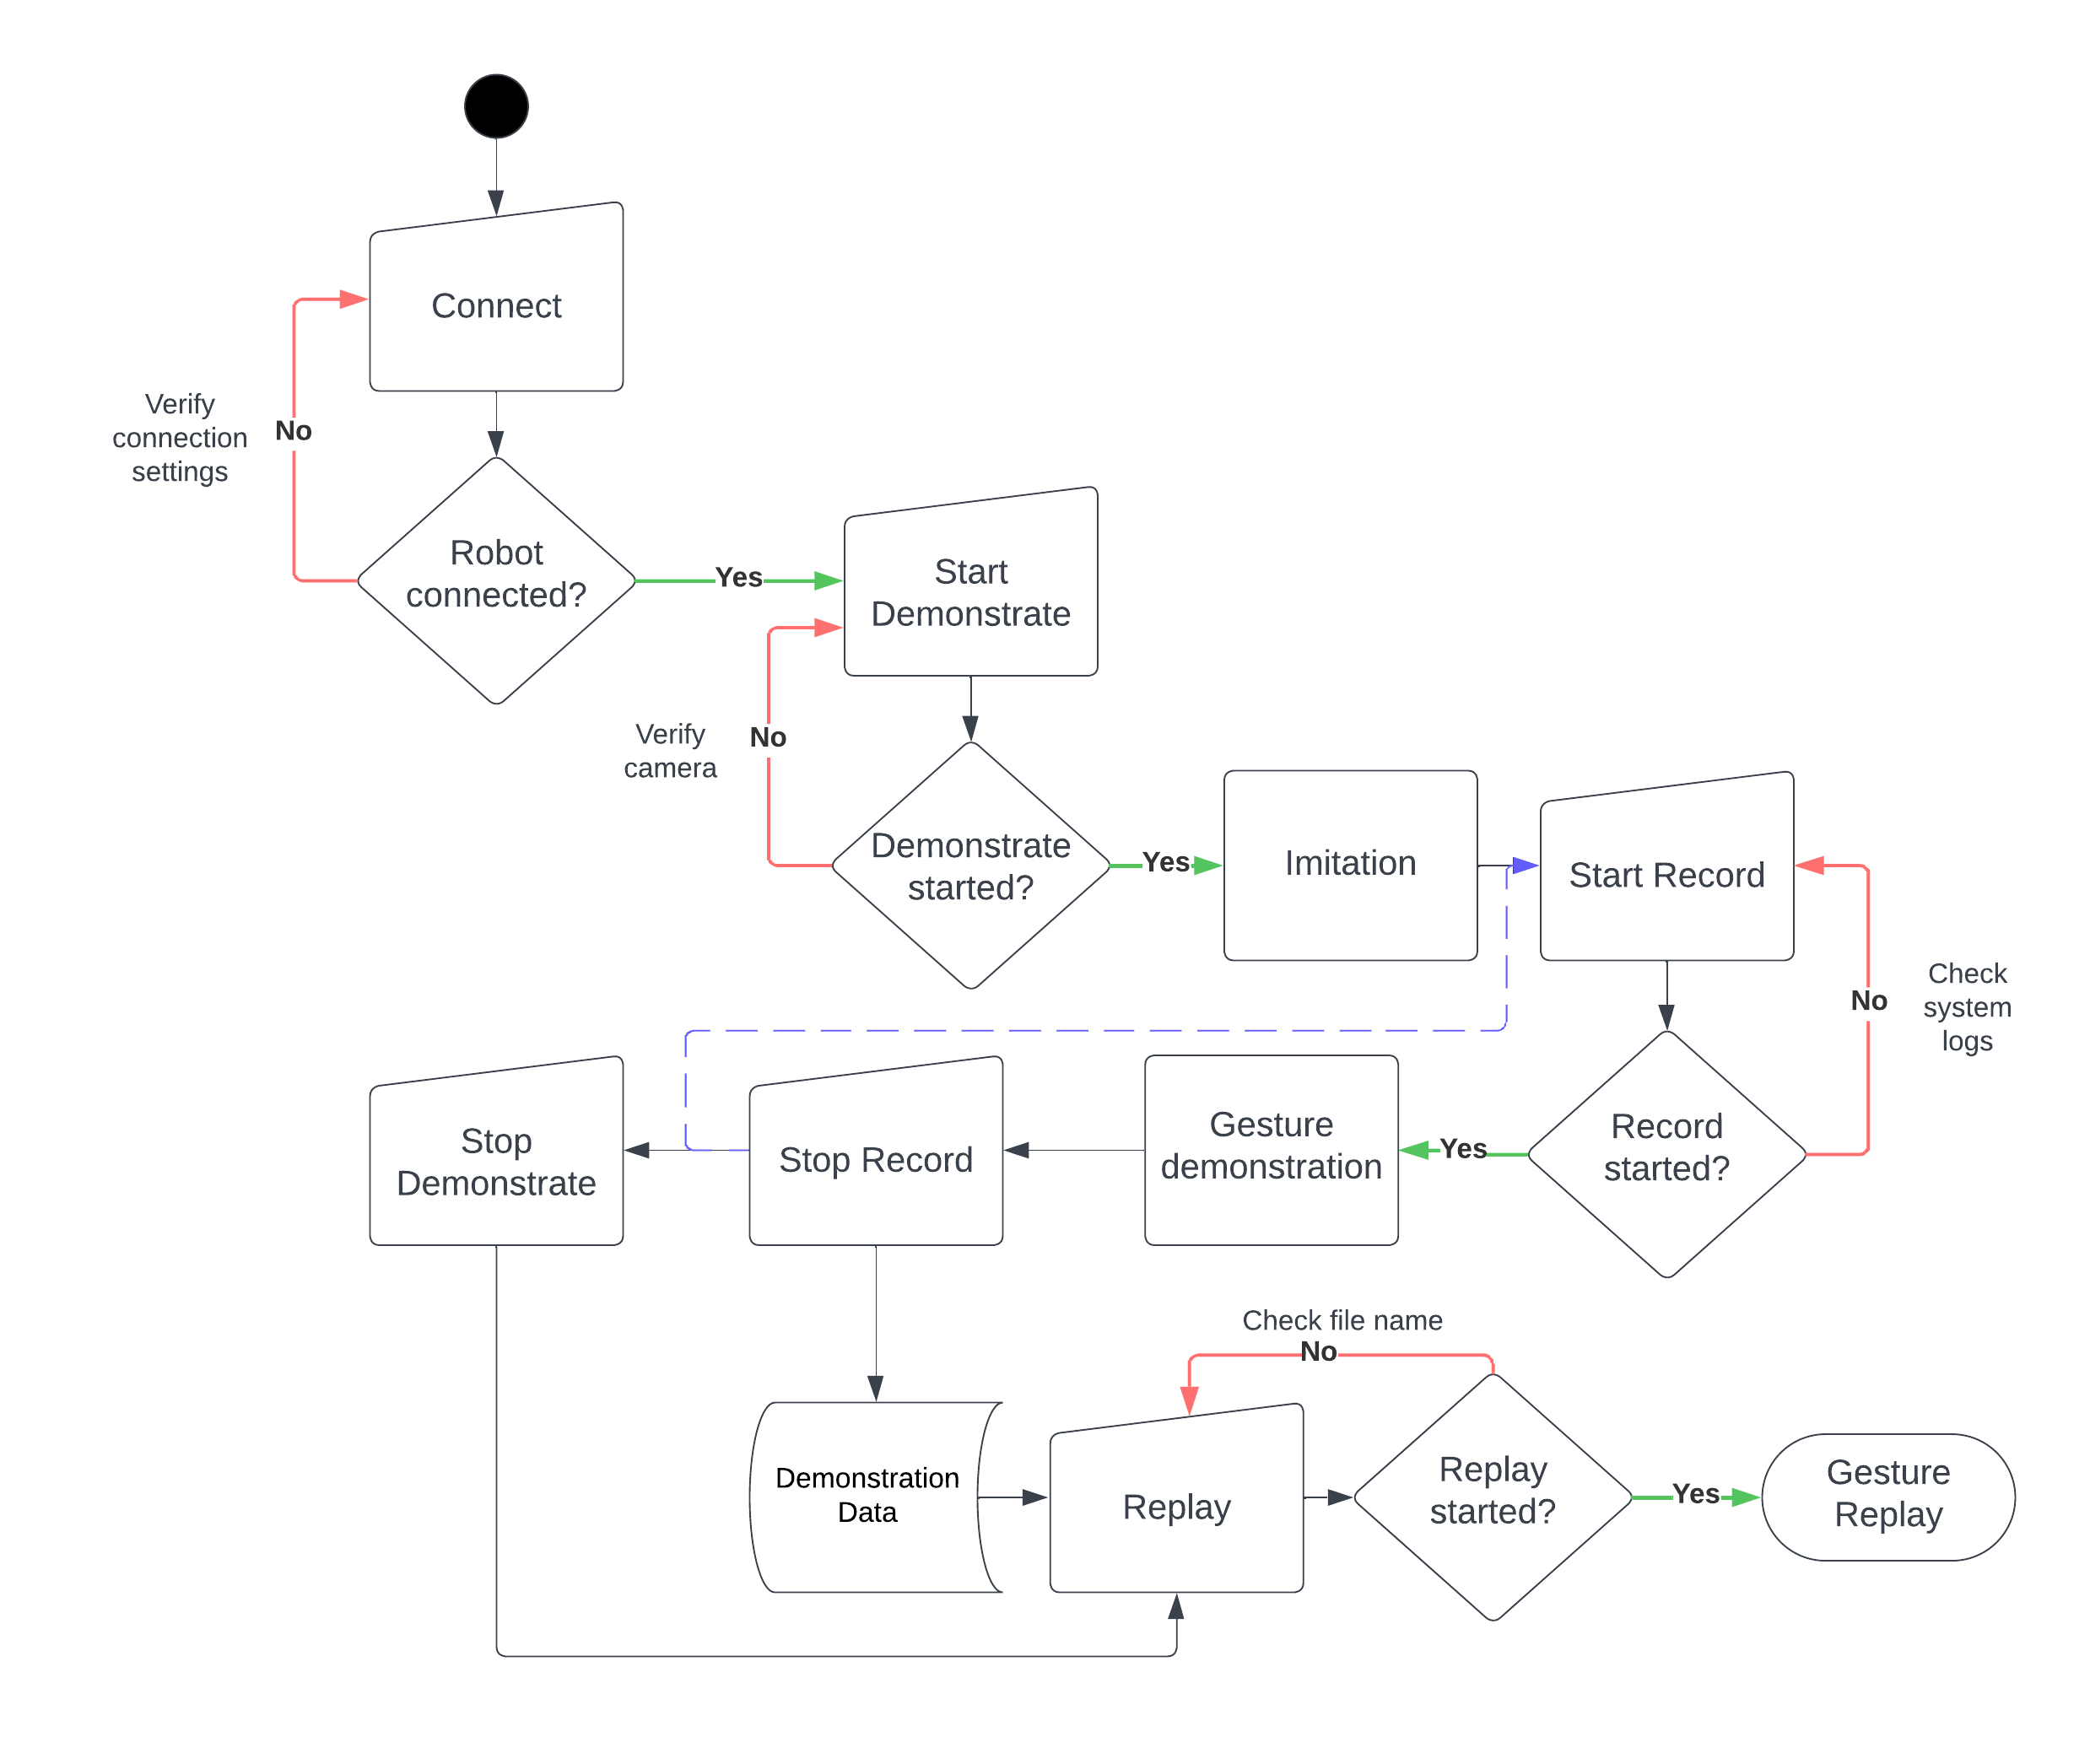
\includegraphics[width=\textwidth]{figures/BehaviouralGraph.png}
    \captionsetup{width=\textwidth}
    \caption{Behavioural graph of the PbD module: The user-centered graph shows an example procedure for demonstrating, recording and replaying. Rectangular boxes represent observable processes, diamond-shaped boxes stand for checks, non-rectangular boxes represent user action. ``Gesture Replay" is the termination element. The blue line indicates the available option of recording multiple demonstrations in one session.}
    \label{fig:behaviouralgraph}
\end{figure}  

\newpage

\section{Module Design}
%===============================================================

\subsection{Design Overview}
The Programming by Demonstration module is implemented in the Python programming language and is designed to process visual and depth images for programming robot gestures by demonstration. Component-based robotic engineering \cite{brugali2010component} is employed using ROS Noetic as the middleware for interprocess communication \cite{Quigleyetal09}. The module consists of three components: \texttt{skeletal\_model}, \texttt{demonstration\_recorder}, and \texttt{demonstration\_gui}. Each component consists of a ROS node. The terms \textit{component} and \textit{node} are used interchangeably throughout the following sections. Same applies to the terms \textit{module} and \textit{package}.


\subsection{Image Source}

The source of the visual and depth images is the ROS driver of an Intel RealSense RGBD camera \cite{realsense_ros} in the case of a live image feed or a custom driver in the case of video. The depth image is aligned with the color image. Both drivers are single-component external modules, \texttt{realsense2\_camera} and \texttt{video\_driver},included as dependencies. Both are implemented as a ROS node, which publishes visual and aligned depth images on two separate topics at a fixed, configurable frequency. This approach stems from the implementation of the Intel RealSense ROS driver \cite{realsense_ros}.

\subsection{Skeletal Model}

The core of the system, the \texttt{skeletal\_model} node, incorporates the following design choices:

\begin{itemize}
    \item Incoming visual and depth images are synchronized, ensuring consistent processing
    \item Synchronized inputs are fed to the MediaPipe deep learning model for human joint pose estimation in cartesian space(\cref{fig:mediapipe})
    \item \(x\) and \(y\) coordinates are retrieved from MediaPipe and concatenated with the \(z\) coordinate from the depth map to generate 3D landmarks.
    \item 3D landmarks are retargeted to Pepper's joints using the GA-LVVJ algorithm \cite{zhang2018real}.
    \item Calculated joint angles are filtered to improve the naturalness of movements. Butterworth and biological motion filters are already implemented and it is possible, though not necessary, to add more (see \cref{sec:anotherfilter}).
    \item Filtered joint angles are fed forward to Pepper’s arm joint controllers for execution. No feedback control is implemented at this level. 
\end{itemize}
\newpage

\begin{figure}[ht!]
    \centering
    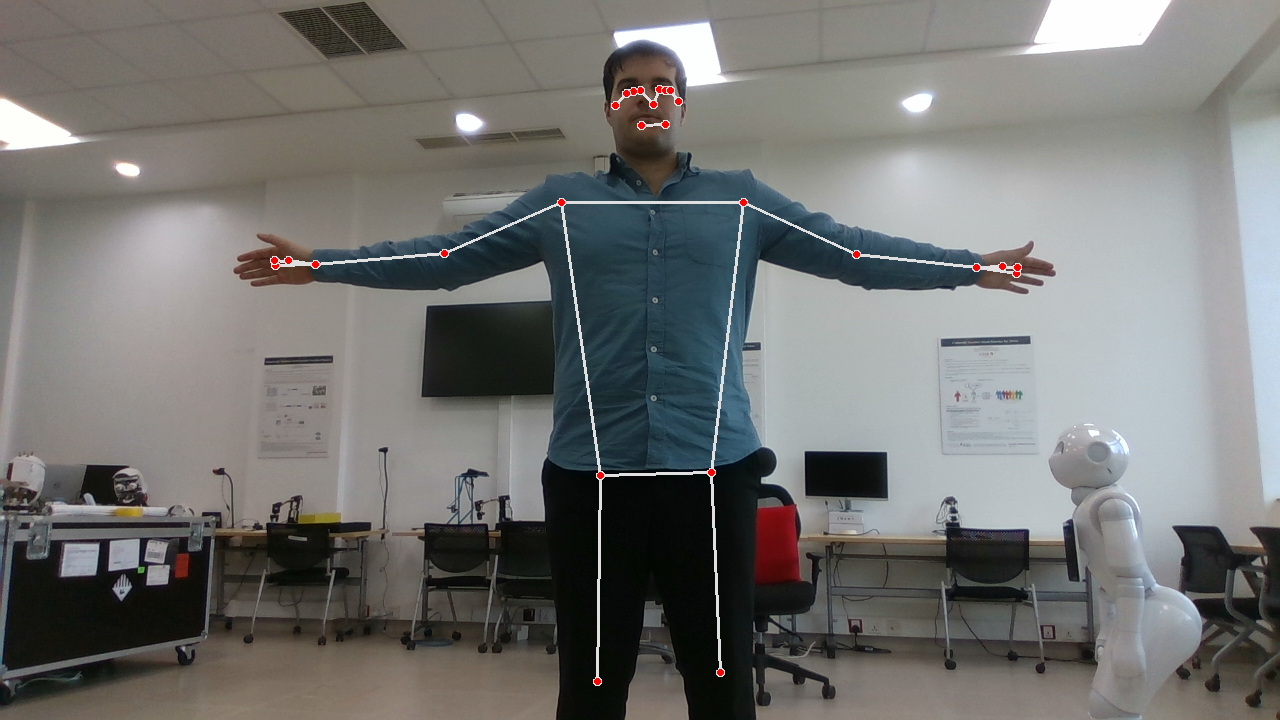
\includegraphics[width=13cm]{figures/mediapipe.png}
    \captionsetup{width=13cm}
    \caption{Skeletal model of the human demonstrator is estimated using Google's MediaPipe pose estimation framework \cite{lugaresi2019mediapipe}.}
    \label{fig:mediapipe}
\end{figure}


\subsection{Demonstration Recorder}
The \texttt{demonstration\_recorder} component comprises several interconnected subcomponents:
\begin{itemize}
    \item \textbf{Data Logger:} Implements functions to start and stop recording time-series data of the robot’s joint angles during demonstrations.
    \item \textbf{Robot Event Handler:} Manages robot control actions such as connecting to the robot, starting, or stopping the demonstration process.
    \item \textbf{User Input Handler:} Processes inputs from the user interface to configure and control the demonstration. The default user interface is the GUI included with this module, but it can be replaced or extended with a user-defined interface for added flexibility (see \cref{sec:anotherinput}).
    \item \textbf{Information Display:} Logs and displays system actions and events in real-time, providing operational feedback. By default, messages are displayed in the GUI. 
    \item \textbf{Demo Recorder:} Coordinates the overall process by managing user inputs and delegating handling of incoming events to the Robot Event Handler or the Data Logger.

\end{itemize}
During operation, user commands are processed by the User Input Handler and shared as events with the Demo Recorder. Depending on the type of event, the Demo Recorder forwards the commands to either the Robot Event Handler or the Data Logger. The outcomes or responses from these subcomponents are then published by the Information Display.

This modular design inspired by \cite{barros2024enhancing} ensures the system is robot-and input-device-agnostic, allowing it to be adapted for use with any robotic platform and to record any type of data, making it flexible for various applications. 

\subsection{Demonstration GUI}

The GUI for the demonstration process (\cref{fig:gui} is implemented using the third-party library PyQt5. Communication with the rest of the system is facilitated by a ROS node, which uses signals and slots \cite{qt_signals_slots} to forward messages to the main Qt application and publish GUI commands to the PbD system. The GUI contains the following elements: 

\begin{itemize}

    \item Entry fields to enter the robot IP and port to connect to the robot
    \item Buttons for capturing user commands (CONNECT, START/STOP DEMONSTRATE, START/STOP RECORD, CLEAR).
    \item A log box to display real-time system logs.
    \item Radio buttons for choosing the filter type 
    \item Check boxes to select the data to be recorded, respectively.
    \item Integration of the MediaPipe feed with the skeletal model, providing a visual representation of the pose estimation process during demonstrations as shown in \cref{fig:mediapipe}.

\end{itemize}


\begin{figure}[ht!]
    \centering
    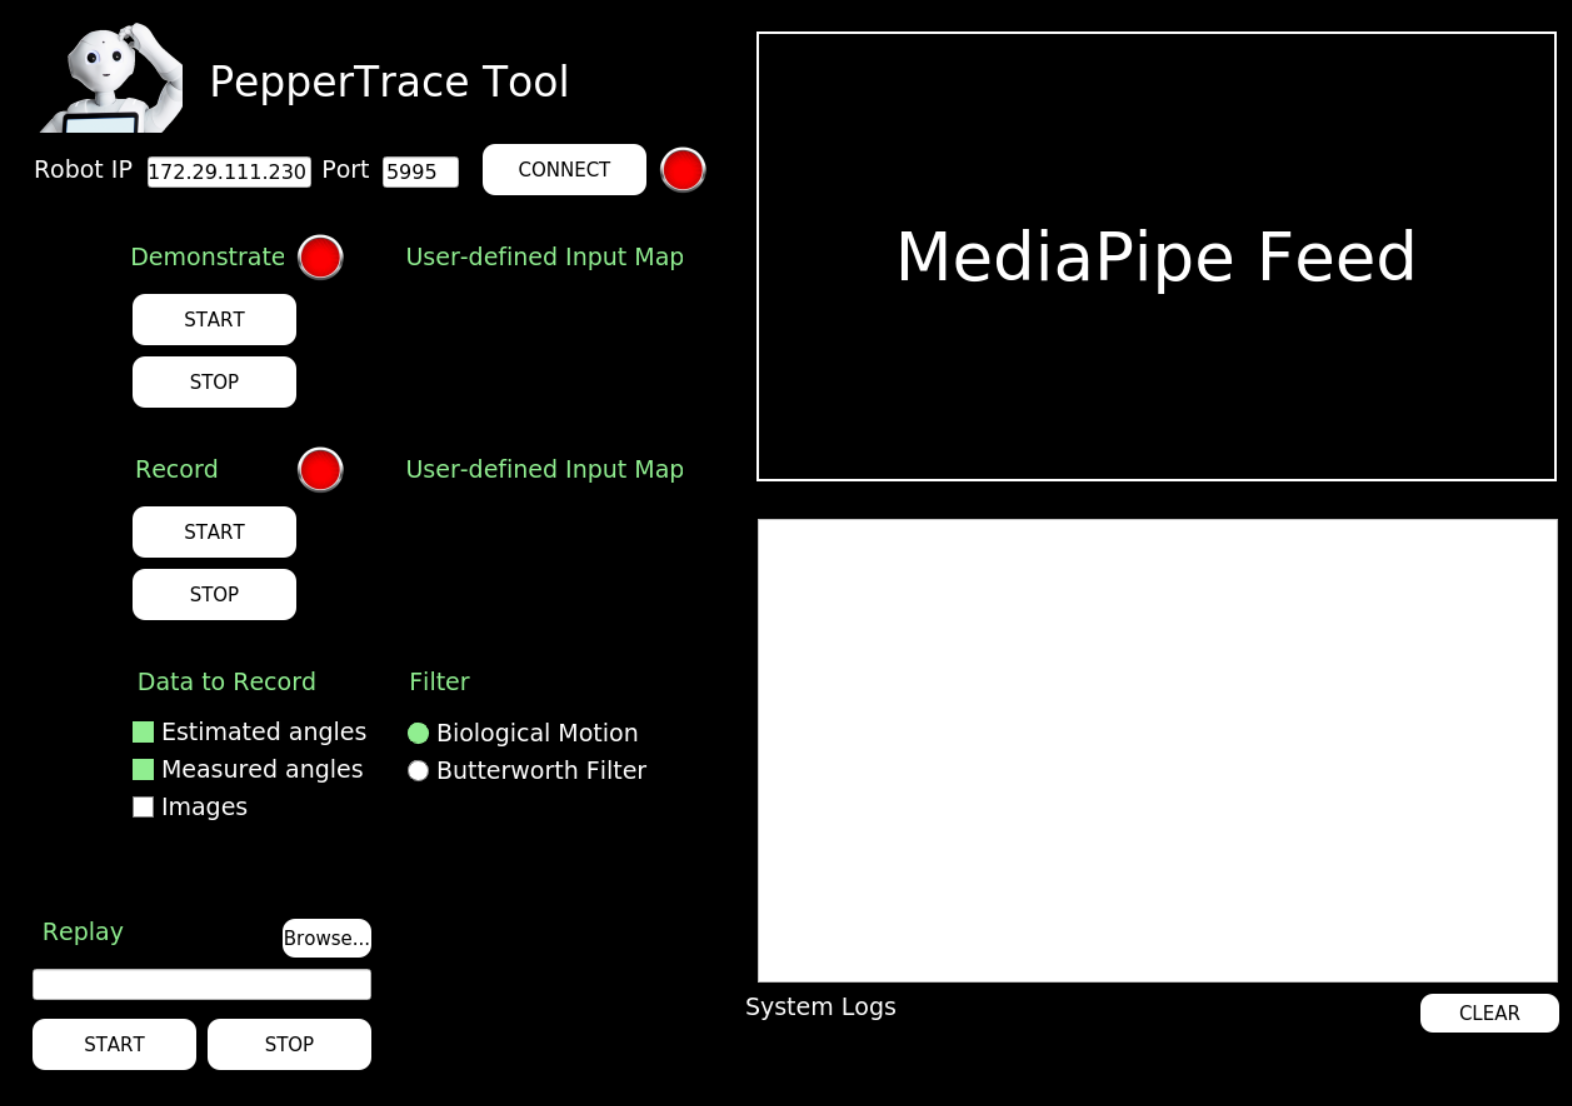
\includegraphics[width=13cm]{figures/peppertrace_gui.png}
    \captionsetup{width=13cm}
    \caption{Graphical User Interface for the Programming by Demonstration system}
    \label{fig:gui}
\end{figure}

\clearpage

\section{Implementation}
\subsection{File Organization \& Purpose}
\hspace{0.5cm}The source code for programming by demonstration is structured into three components: \\
\texttt{skeletal\_model}, \texttt{demonstration\_recorder} and \texttt{demonstration\_gui}. Each of these components operates as a ROS node, with distinct roles: retargeting estimated human joint positions to Pepper's joint angles, recording demonstration data, and providing a GUI as the user interface for the PbD system. Each component contains the following elements: 
\begin{itemize}
    \item \textbf{/config folder:} contains configuration files in the JSON format. These files store parameters and settings that can be adjusted to modify the behavior of the component without changing the source code.
    \item \textbf{/launch folder :} includes ROS launch files that automate the startup process of ROS nodes and set parameter values.
    \item \textbf{/src folder:} Source files are divided into one application and multiple implementation files. The rationale behind the nomenclature is that the user of a node does not need to know the implementation details to use it as an application. As a rule, each implementation file contains one Python class, according to the name of the file. The inclusion of an \texttt{\_\_init.py\_\_.py} file signals to Python that the directory should be treated as a package with importable scripts \cite{betterstack_initpy}
    \item \textbf{CMakeLists.txt file:} provides build instructions for the component using CMake, which is integrated with ROS through the catkin build system \cite{catkin_docs}.
    \item \textbf{README.md file:} offers documentation and usage instructions for the component. 
\end{itemize}

The \texttt{demonstration\_gui} additionally contains an \texttt{images} folder, which can contain any number of image files, typically in the \texttt{*.png} format. These images are displayed in the GUI as logos or status identifiers. 

Along with the component directories, the root directory of the module contains a package.xml file, which includes meta-information about the ROS package, e.g the package name, version, description, maintainers, license, and dependencies on other ROS packages. It also contains the top level CMakeLists.txt and README.md files for module-level build instructions and documentation, respectively. 

\newpage
\cref{fig:dirtree_structure} shows the file structure of the \texttt{programming\_by\_demonstration} package.


\begin{figure}[H]
    \renewcommand*\DTstyle{\ttfamily\scriptsize}
    \renewcommand{\DTbaselineskip}{0.7em} % Reduce vertical spacing
    \dirtree{%
    .1 programming\_by\_demonstration.
    .2 demonstration\_gui.
    .3 config.
    .4 demonstration\_gui\_configuration.json.
    .3 images.
    .4 *.png.
    .3 launch.
    .4 demonstration\_gui.launch.
    .3 src.
    .4 \_\_init\_\_.py.
    .4 demonstration\_gui\_application.py.
    .4 demonstration\_gui\_elements\_implementation.py.
    .4 demonstration\_gui\_logic\_implementation.py.
    .4 demonstration\_gui\_ros\_interface\_implementation.py.
    .3 CMakeLists.txt.
    .3 README.md.
    .2 demonstration\_recorder.
    .3 config.
    .4 demonstration\_recorder\_configuration.json.
    .3 launch.
    .4 demonstration\_recorder.launch.
    .3 src.
    .4 \_\_init\_\_.py.
    .4 demonstration\_recorder\_application.py.
    .4 demonstration\_recorder\_data\_logger\_implementation.py.
    .4 demonstration\_recorder\_demo\_recorder\_implementation.py.
    .4 demonstration\_recorder\_information\_display\_implementation.py.
    .4 demonstration\_recorder\_robot\_event\_handler\_implementation.py.
    .4 demonstration\_recorder\_recorder\_ros\_utils.py.
    .4 demonstration\_recorder\_rosbag\_recorder\_implementation.py.
    .4 demonstration\_recorder\_states\_and\_events\_implementation.py.
    .4 demonstration\_recorder\_user\_input\_handler\_implementation.py.
    .3 CMakeLists.txt.
    .3 README.md.
    .2 skeletal\_model.
    .3 config.
    .4 skeletal\_model\_configuration.json.
    .3 launch.
    .4 skeletal\_model.launch.
    .3 src.
    .4 \_\_init\_\_.py.
    .4 skeletal\_model\_application.py.
    .4 skeletal\_model\_estimation\_implementation.py.
    .4 skeletal\_model\_filters\_implementation.py.
    .4 skeletal\_model\_retargeting\_implementation.py.
    .3 CMakeLists.txt.
    .3 README.md.
    .2 CMakeLists.txt.
    .2 package.xml.
    .2 README.md.
    }
\captionsetup{width=\textwidth}
\caption{Directory structure of the PbD module consisting of three components each with config, launch, src folders and CMakeLists.txt and README.md files. The root directory also includes the package.xml file. }
\label{fig:dirtree_structure}
\end{figure}

\newpage



\vspace*{0.5em}
\subsection{Skeletal Model Implementation}

\subsubsection*{Python Classes}
The \texttt{skeletal\_model} component is implemented with several classes that achieve the functionality depicted in \cref{fig:computationalgraph}. The class diagram is depicted in \cref{fig:skeletaluml}.

\begin{itemize}
    \item \textbf{SkeletalModelEstimation - main implementation:} 
    \begin{itemize}
        \item uses synchronized ROS \texttt{message\_filters} subscribers to receive visual and depth images
        \item processes images in a callback: gets 3D landmarks in cartesian space in the camera frame from MediaPipe and depth map, runs retargeting and filtering functions and publishes the angles on a ROS topic. Numerical quantities like 3D landmarks and joint angles are processed as Numpy arrays \cite{harris2020array}. 
        \item the current image with skeletal model overlay as in \cref{fig:mediapipe} is published on a ROS topic in the main node loop. A mutex lock prevents simultaneous access to the current image from image callback and main loop. 
    \end{itemize}
    \item \textbf{DataFilter - filter implementation:}
    \begin{itemize}
        \item Uses a Numpy array as the data type for the filter window. 
        \item Saves points in the window and applies filter to it when it is full and a new point arrives. The specific filtering function that is called depends on the value of the filter\_type attribute  of type String. The class contains a setter method for this attribute. 
    \end{itemize}
    \item \textbf{HumanToHumanoidRetargeting - retargeting implementation:}
    \begin{itemize}
        \item main function get\_angles returns a Numpy array of Pepper joint angles from 3D landmarks on the human body
        \item class contains helper functions for calculation of each joint angle for both arms
    \end{itemize}
\end{itemize}


\subsubsection*{Configuration File}
The configuration file is named \texttt{skeletal\_model\_configuration.json}. It contains a list of key-value pairs that determine the operation of the node. 

% Table of 3 x 4 with the following headers: Key, Value, Description
\begin{longtable}[c]{|l|l|p{5cm}|}
    \caption{Configuration file for the skeletal model} \label{tab:config_file}\\
    \hline
    \rowcolor{gray!30}
    \small{\textbf{Key}} & \small{\textbf{Value Type}} & \small{\textbf{Description}} \\ \hline
    \endhead % header for subsequent pages
    
    \small{\texttt{camera\_intrinsics}} & \small{\texttt{List of lists of floats}}  & \small{Contains matrix with camera's intrinsic parameters} \\ \hline
    \small{\texttt{image\_width}} & \small{\texttt{String}} & \small{Specifies the width of color and depth used.} \\ \hline
    \small{\texttt{image\_height}} & \small{\texttt{String}} & \small{Specifies the width of color and depth images used.} \\ \hline
    \small{\texttt{color\_image\_topic}} & \small{\texttt{String}} & \small{Topic where color image feed is published. } \\ \hline
    \small{\texttt{depth\_image\_topic}} & \small{\texttt{String}}& \small{Topic where aligned depth image feed is published. } \\ \hline
    \small{\texttt{left\_arm\_command\_topic}} & \small{\texttt{String}} & \small{Topic to publish control signal for left arm.} \\ \hline
    \small{\texttt{right\_arm\_command\_topic}} & \small{\texttt{String}} & \small{Topic to publish control signal for right arm.} \\ \hline
    \small{\texttt{gui\_commands\_topic}} & \small{\texttt{String}} & \small{Topic to receive user commands to change system behavior (e.g. filter)} \\ \hline
    \small{\texttt{skeletal\_model\_feed\_topic}} & \small{\texttt{String}} & \small{Topic to publish images with skeletal model overlay.} \\ \hline
\end{longtable}

\subsection*{Input File}
During offline usage, a video file in the format \texttt{.bag} serves as input to the system. It should be placed in the \texttt{skeletal\_model/data} folder and be called \texttt{video\_input.bag}. It should contain depth information. The \texttt{src} folder contains an utility script to record a video with the Intel RealSense camera. 

\subsection*{Output Data File}
There is no output data file for the actuator test. The result of the angle calculation from the skeletal model is published on the skeletal model image feed and arm controller topics. 


\subsubsection*{Topics Subscribed}
\begin{longtable}[c]{|l|l|l|}
    \caption{Topics subscribed by the skeletal\_model node.} \label{tab:Published_topics} \\
    \hline
    \rowcolor{gray!30}
    \footnotesize{\textbf{Topic}} & \footnotesize{\textbf{Message Type}} \\ \hline
    \endhead % header for subsequent pages
    
    \footnotesize{\texttt{/camera/color/image\_raw}} & \footnotesize{\texttt{sensor\_msgs/Image}} \\ \hline
    \footnotesize{\texttt{/camera/aligned\_depth\_to\_color/image\_raw}} & \footnotesize{\texttt{sensor\_msgs/Image}} \\ \hline
    \footnotesize{\texttt{/gui/commands}} & \footnotesize{\texttt{std\_msgs/String}} \\ \hline

\end{longtable}
\newpage 
\subsubsection*{Topics Published}

\begin{longtable}[c]{|l|l|l|}
    \caption{Topics published by the skeletal\_model node.} \label{tab:Published_topics} \\
    \hline
    \rowcolor{gray!30}
    \footnotesize{\textbf{Topic}} & \footnotesize{\textbf{Message Type}} \\ \hline
    \endhead % header for subsequent pages
    
    \footnotesize{\texttt{/mediapipe/image\_feed}} & \footnotesize{\texttt{sensor\_msgs/Image}} \\ \hline
    \footnotesize{\texttt{/pepper\_dcm/LeftArm\_controller/command}} & \footnotesize{\texttt{trajectory\_msgs/JointTrajectory}} \\ \hline
    \footnotesize{\texttt{/pepper\_dcm/RightArm\_controller/command}} & \footnotesize{\texttt{trajectory\_msgs/JointTrajectory}} \\ \hline

\end{longtable}

\begin{figure}[H]
    \centering
    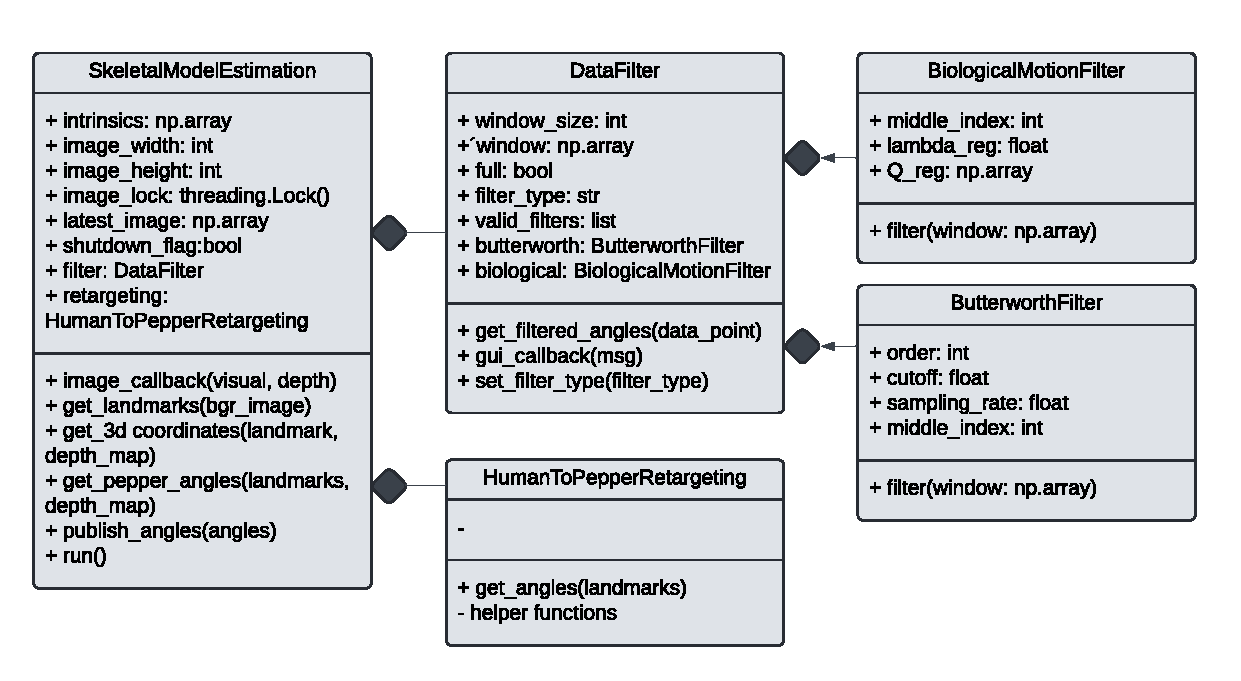
\includegraphics[width=\linewidth]{figures/skeletal_model.pdf}
    \caption{UML class diagram for the skeletal model component. Class visualization contains name, attributes and methods from top to bottom. Class relationships are of composition (filled diamond), as classes where symbol ends instantiate the others as attributes.}
    \label{fig:skeletaluml}
\end{figure}


\newpage
\subsection*{Launch File}
The \texttt{skeletal\_model.launch} launch file is used to launch the skeletal\_model node. The required parameter is set to true.
The same file also launches the ROS driver for the camera. In this implementation it is the ROS driver for the Intel RealSense camera with launch parameters:

\begin{itemize}
    \item \texttt{align\_depth}: whether to align depth image to color image (possible values: true, false ; default: true).
    \item \texttt{color\_fps}: frequency that images are captured in frames-per-second (possible values: 6,15,30 ; default: 15).
    \item \texttt{color\_width}: specifies width of the color image, depth image is aligned to this width (possible values: see \cref{fig:resolutions}, default: 1280).  
    \item \texttt{color\_height}: specifies height of the color image, depth image is aligned to this height (possible values: see \cref{fig:resolutions}, default: 720).  
\end{itemize}

\begin{figure}[H]
    \centering
    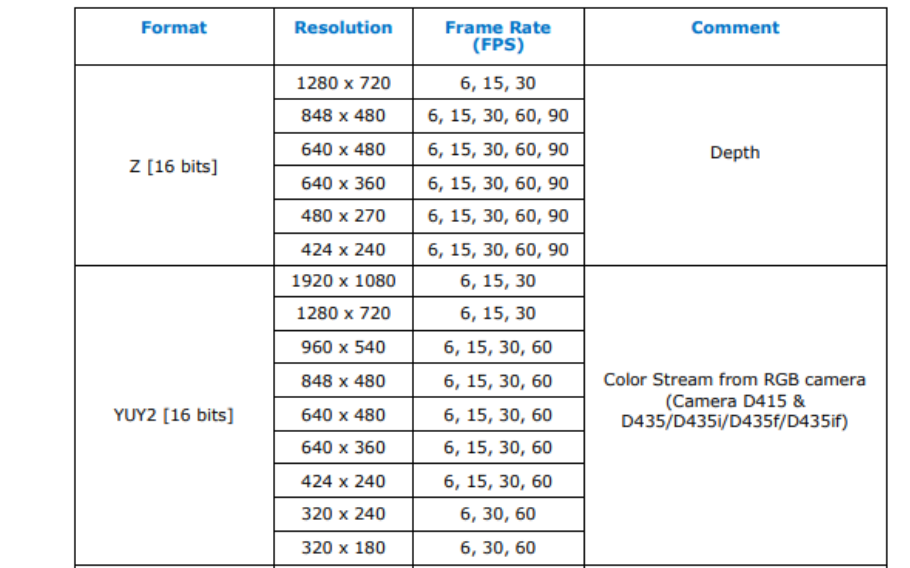
\includegraphics[width=\textwidth]{figures/realsenseresolutions.png}
    \caption{Table with available image formats using USB 3.1 Gen 1 and the Intel RealSense D435 \cite{intel_realsense_d435}}
    \label{fig:resolutions}
\end{figure}


%%%%%%%%%%%%%%%%%%%%%%%%%%%%%%%%%%%%%%%%%%%%%%%%%%%%%%%%%%%%%%%%%%%%%%%%%%%%%%%%%%%%%%%%%%%%%%%%%%%%%%%%%%%%%%%%%%%%%%%%%%%%
\newpage
\subsection{Demonstration Recorder Implementation}

\subsubsection*{Python Classes}
The \texttt{demonstration\_recorder} component is implemented with several classes that achieve the functionality depicted in \cref{fig:behaviouralgraph}. The class diagram is depicted in \cref{fig:recorderuml}.

\begin{itemize}
    \item \textbf{Event, EventType, States, Commands - event implementation (\cref{fig:states}):} 
    \begin{itemize}
        \item The Event class defines an event with an event type, a command and optional arguments.
        \item The EventType is defined as a Python Enum and specifies DATA\_LOGGING, ROBOT\_CONTROL and TERMINATE as possible types.
        \item DataLoggerCommands, DataLoggerStates, RobotCommands and RobotStates are all Enums and define the available states and commands for the data logger and the robot event handler.
    \end{itemize}
    \item \textbf{GuiInputHandler - user input implementation:} 
    \begin{itemize}
        \item Processes user input from the GUI buttons in a ROS subscriber callback by posting events to an event queue shared with the DemoRecorder.
        \item It contains the input map object as an attribute that the user can define if adapting this class to another input device. The keys are ``Demonstrate and ``Record" and the values represent the corresponding inputs for Start and Stop. In the current implementation, these are the GUI buttons, but in a custom implementation they can refer to e.g. the buttons on a mouse, see \cref{sec:anotherinput}.
    \end{itemize}
    \item \textbf{PepperRobotEventHandler - robot interface implementation:}
    \begin{itemize}
        \item Contains handle\_event function that calls other class methods for connecting/disconnecting the robot and starting/stopping demonstrate mode. 
        \item Connection and demonstrate processes are started in subprocesses that execute ROS launch files.
        \item A monitor function checks whether the demonstrate process exits and reports an exit directly to the user via the GUI by publishing a message on a ROS topic.
    \end{itemize}
    \item \textbf{PepperROS1DataLogger - data recording implementation:}
    \begin{itemize}
        \item Contains handle\_event function that calls other class methods for starting/stopping data logging, starting/stopping replay and setting the data, and indirectly the ROS topics, that should be recorded. 
        \item Record and replay processes are started in subprocesses using \texttt{rosbag record} and \texttt{rosbag play} respectively. 
        \item A monitor function checks whether the replay process exits and sets the state of the class to IDLE on stopped replay.
        \item The set\_topics function receives types of data to record and maps it to the respective topics, setting the topic\_list attribute that the record process uses to record the topics.  
    \end{itemize}
    \newpage
    \item \textbf{GuiInformationDisplay - information display implementation:}
    \begin{itemize}
        \item This class uses a ROS publisher to publish information from the other systems to the GUI. 
        \item It also publishes the input map on startup, prompted by the DemoRecorder. 
    \end{itemize}
    \item \textbf{DemoRecorder - orchestrating implementation:}
    \begin{itemize}
        \item Implements the main loop which keeps the component running and delegates incoming tasks from the user input handler to the data logger or the robot event handler. 
        \item The information returned by both event handling systems is forwarded to the information display for informing the user through the GUI. 
        \item At startup, it publishes the input map for display in the GUI and passes the event queue to the user input, which becomes shared. 
        \item A terminate event triggered by user input will stop the system. This can be included, see \cref{sec:anotherinput}, but out of the box works by entering Ctrl-C in the terminal. 
    \end{itemize}
\end{itemize}

\begin{figure}[htb]
    \centering
    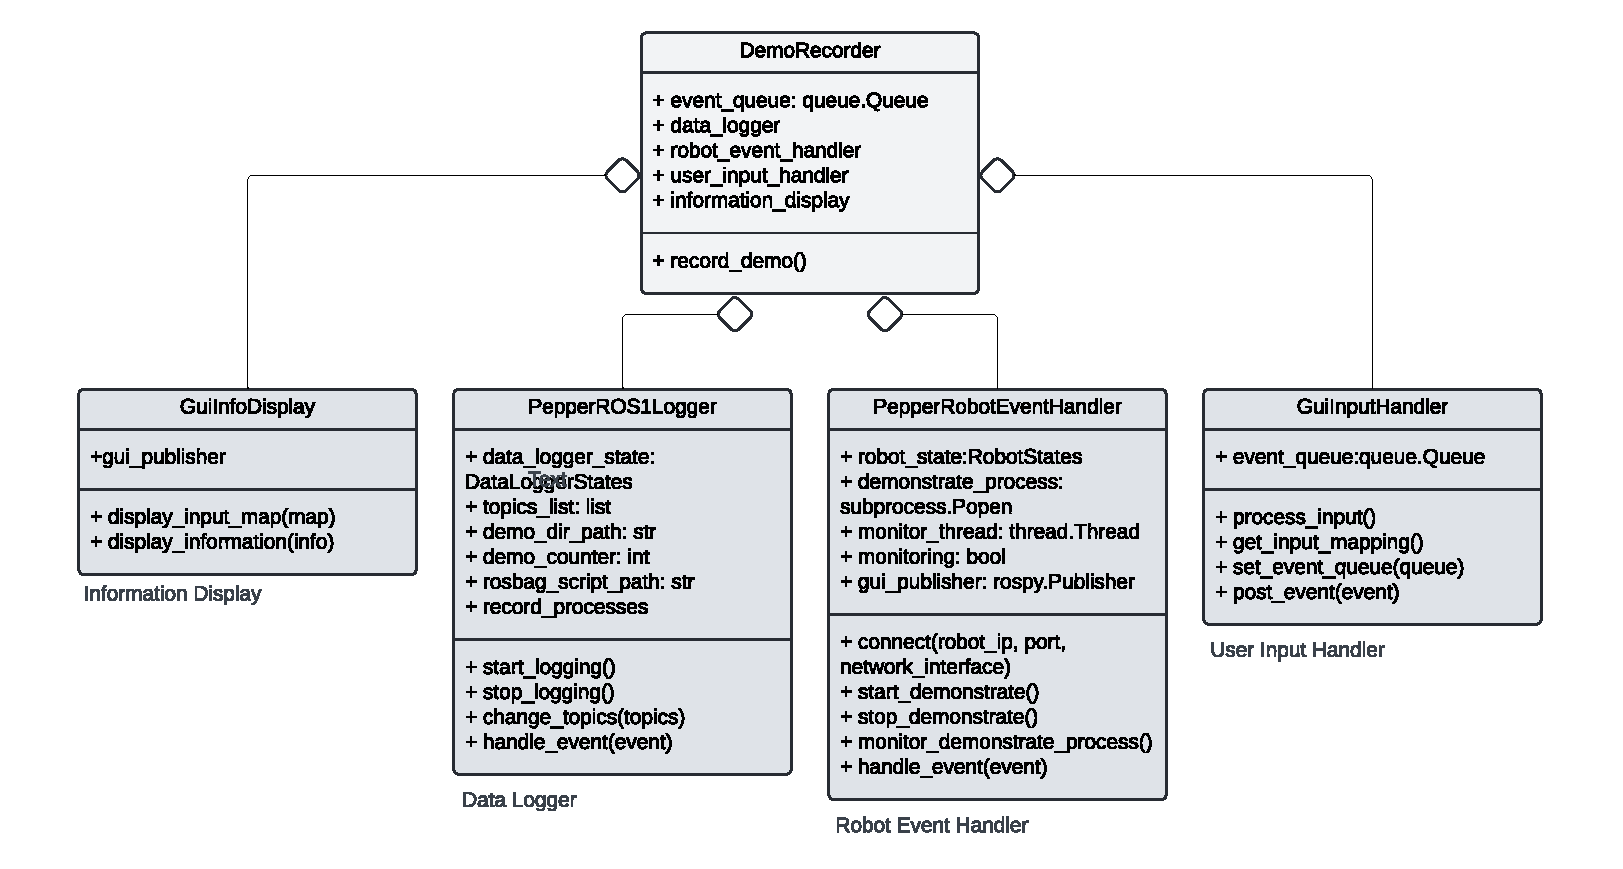
\includegraphics[width=\linewidth]{figures/DemoRecorder.pdf}
    \caption{UML class diagram for the demonstration recorder component. Class visualization contains name, attributes and methods from top to bottom. Class instances are aggregated by the DemoRecorder (unfilled diamond)}
    \label{fig:recorderuml}
\end{figure}

\begin{figure}[htb]
    \centering
    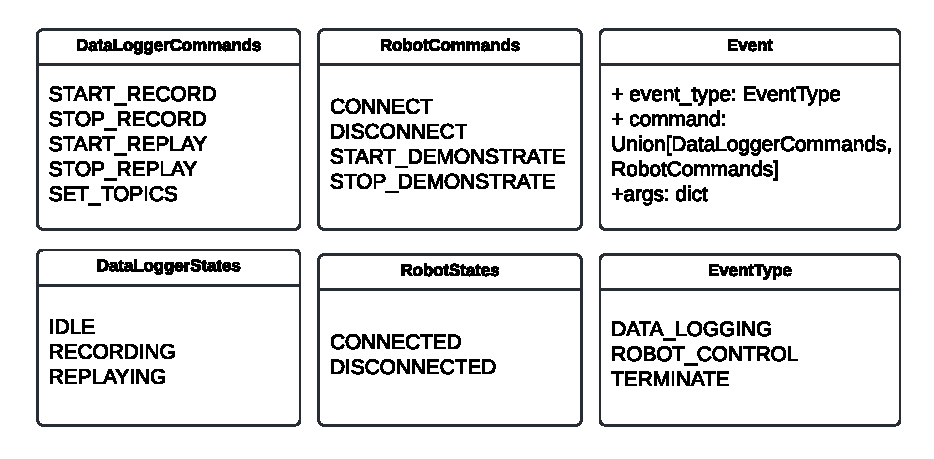
\includegraphics[width=\linewidth]{figures/states.pdf}
    \caption{Event types, states and enums as Python Enums, Event as a Python class}
    \label{fig:states}
\end{figure}


\subsubsection*{Configuration File}
The configuration file is named \texttt{demonstration\_recorder\_configuration.json}. It contains a list of key-value pairs that determine the operation of the node. The \texttt{.} here denote nested parameters in the json structure.

% Table of 3 x 4 with the following headers: Key, Value, Description
\begin{longtable}[c]{|l|l|p{7cm}|}
    \caption{Configuration file for the demonstration recorder} \label{tab:config_file}\\
    \hline
    \rowcolor{gray!30}
    \small{\textbf{Key}} & \small{\textbf{Value Type}} & \small{\textbf{Description}} \\ \hline
    \endhead % header for subsequent pages
    
    \small{\texttt{data\_logger.topics\_list}} & \small{\texttt{List of strings}}  & \small{Specifies the list of topics to be recorded during demonstration.} \\ \hline
    \small{\texttt{data\_logger.data\_dir}} & \small{\texttt{String}} & \small{Specifies the root directory where the bag files will be stored.} \\ \hline
    \small{\texttt{data\_logger.demo\_name}} & \small{\texttt{String}} & \small{Specifies the name of the demonstration and will be the directory inside data\_dir where the bag files will be stored.} \\ \hline
    \small{\texttt{gui\_system\_logs\_topic}} & \small{\texttt{String}} & \small{Topic where messages to be displayed in the GUI are published.} \\ \hline
    \small{\texttt{gui\_commands\_topic}} & \small{\texttt{String}}& \small{Topic to receive user commands to change behavior (e.g. start recording).} \\ \hline
    \small{\texttt{skeletal\_model\_feed\_topic}} & \small{\texttt{String}} & \small{Topic to publish images with skeletal model overlay.} \\ \hline
\end{longtable}



\subsection*{Input File}
There is no input file for the demonstration\_recorder node. The demonstrations are recorded from messages that are sent on relevant topics in the ROS system. 


\subsection*{Output Data File}
Output .bag files comprise recorded demonstration data saved in \texttt{<data\_dir>/<demo\_name>} on the local machine. 

\newpage
\subsubsection*{Topics Subscribed}
\begin{longtable}[c]{|l|l|l|}
    \caption{Topics subscribed by the demonstration\_recorder node.} \label{tab:Published_topics} \\
    \hline
    \rowcolor{gray!30}
    \footnotesize{\textbf{Topic}} & \footnotesize{\textbf{Message Type}} \\ \hline
    \endhead % header for subsequent pages
    
    \footnotesize{\texttt{/gui/commands}} & \footnotesize{\texttt{std\_msgs/String}} \\ \hline
    \footnotesize{\texttt{/joint\_states}*} & \footnotesize{\texttt{sensor\_msgs/JointState}} \\ \hline
    \footnotesize{\texttt{/pepper\_dcm/LeftArm\_controller/command}*} & \footnotesize{\texttt{trajectory\_msgs/JointTrajectory}} \\ \hline
    \footnotesize{\texttt{/pepper\_dcm/RightArm\_controller/command}*} & \footnotesize{\texttt{trajectory\_msgs/JointTrajectory}} \\ \hline

\end{longtable}
{\footnotesize *These topics are examples of topics that can be recorded by the data\_logger with rosbag.}

\subsubsection*{Topics Published}

\begin{longtable}[c]{|l|l|l|}
    \caption{Topics subscribed by the demonstration\_recorder node.} \label{tab:Published_topics} \\
    \hline
    \rowcolor{gray!30}
    \footnotesize{\textbf{Topic}} & \footnotesize{\textbf{Message Type}} \\ \hline
    \endhead % header for subsequent pages
    \footnotesize{\texttt{/gui/system\_logs}} & \footnotesize{\texttt{std\_msgs/String}} \\ \hline
\end{longtable}

\subsection*{Launch File}
The \texttt{demonstration\_recorder.launch} launch file is used to launch the demonstration recorder node. No launch parameters are required. 

%%%%%%%%%%%%%%%%%%%%%%%%%%%%%%%%%%%%%%%%%%%%%%%%%%%%%%%%%%%%%%%%%%%%%%%%%%%%%%%%%%%%%%%%%%%%%%%%%%%%%%%5
\subsection{Demonstration GUI Implementation}

\subsubsection*{Python Classes}
The \texttt{demonstration\_gui} component is implemented with several classes that achieve the design and functionality of the GUI (\cref{fig:gui}). The class diagram is depicted in \cref{fig:guiuml}.

\begin{itemize}
    \item \textbf{Ui\_MainWindow - visual elements implementation:} 
    \begin{itemize}
        \item setupUi function instantiates all elements that can be seen in the GUI such as labels, text boxes and buttons. 
        \item retranslateUi function sets the text for all the elements and translates them to their specified position in the main window.
        \item  This Python class is generated by PyQt5 from the \texttt{.ui} file generated with the Qt Designer application, where the GUI was put together.  
    \end{itemize}
    \item \textbf{RosThread and RosNode - ROS interface implementation:}
    \begin{itemize}
        \item The Qt application needs to run in the main thread, so RosThread inherits from QThread to spin a ROS node in a secondary thread
        \item The RosNode class contains this node which has two subscribers, one for system logs and another for the skeletal model image feed, and one publisher for system commands. It forwards incoming ROS messages to the MainWindow via PyQt signals and publishes commands from the MainWindow to a ROS topic
    \end{itemize}
    \item \textbf{MainWindow - GUI logic implementation:}
    \begin{itemize}
        \item This class instantiates both the others. Having access to the GUI elements from Ui\_MainWindow, it connects the buttons to the class methods that enable the desired functionality, e.g. sending commands to the RosThread instance for publishing. 
        \item Incoming messages from the RosThread are processed by PyQt slots, which display the logs in the system logs box or the skeletal model image feed above it.
        \item It also changes the color of status symbols on the GUI, i.e. the light icons, between green and red depending on log messages from the other components of the Programming by Demonstration system. 
    \end{itemize}
\end{itemize}

\begin{figure}[htb]
    \centering
    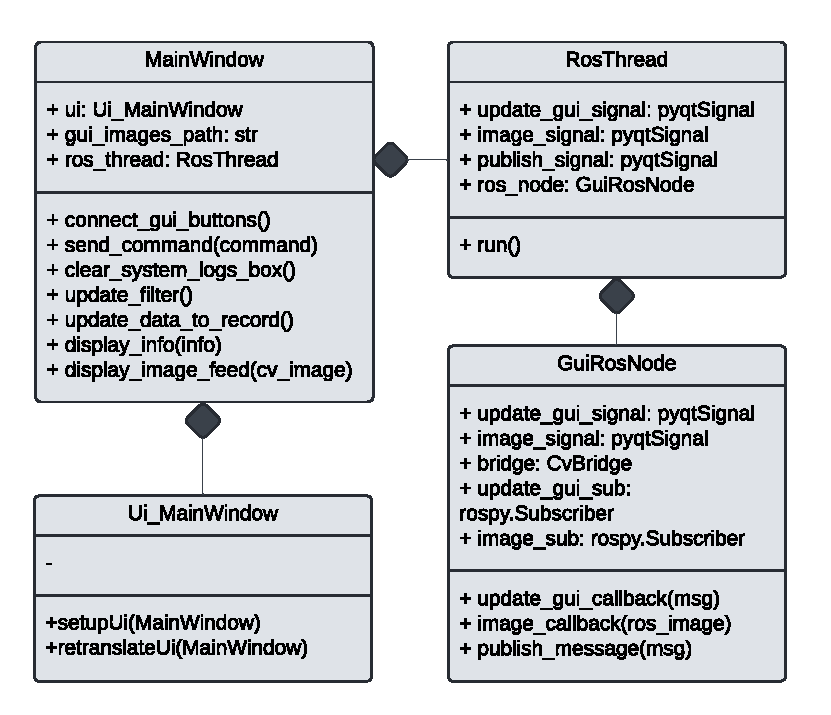
\includegraphics[width=0.9\linewidth]{figures/gui.pdf}
    \caption{UML class diagram for the demonstration gui component. Class visualization contains name, attributes and methods from top to bottom. Class relationships are of composition (filled diamond), as classes where symbol ends instantiate the others as attributes.}
    \label{fig:guiuml}
\end{figure}


\subsubsection*{Configuration File}
The configuration file is named \texttt{demonstration\_gui\_configuration.json}. It contains a list of key-value pairs that determine the operation of the node. The \texttt{.} here denote nested parameters in the json structure.

% Table of 3 x 4 with the following headers: Key, Value, Description
\begin{longtable}[c]{|l|l|p{7cm}|}
    \caption{Configuration file for the demonstration GUI} \label{tab:config_file}\\
    \hline
    \rowcolor{gray!30}
    \small{\textbf{Key}} & \small{\textbf{Value Type}} & \small{\textbf{Description}} \\ \hline
    \endhead % header for subsequent pages
    \small{\texttt{gui\_system\_logs\_topic}} & \small{\texttt{String}} & \small{Topic where messages to be displayed in the GUI are published.} \\ \hline
    \small{\texttt{gui\_commands\_topic}} & \small{\texttt{String}} & \small{Topic to publish user commands to change behavior in other subsystems (e.g. filter in \texttt{skeletal\_model}).} \\ \hline
    \small{\texttt{skeletal\_model\_feed\_topic}} & \small{\texttt{String}} & \small{Topic to publish images with skeletal model overlay.} \\ \hline
\end{longtable}

\subsection*{Input File}
There is no input file for the demonstration\_gui node. It responds to user input which it passes on to the rest of the PbD system. 

\subsection*{Output Data File}
There is no output data file demonstration\_gui node. System logs are flushed to the terminal and the GUI itself.

\subsubsection*{Topics Subscribed}
\begin{longtable}[c]{|l|l|l|}
    \caption{Topics subscribed by the demonstration\_gui node.} \label{tab:Published_topics} \\
    \hline
    \rowcolor{gray!30}
    \footnotesize{\textbf{Topic}} & \footnotesize{\textbf{Message Type}} \\ \hline
    \endhead % header for subsequent pages
    
    \footnotesize{\texttt{/gui/system\_logs}} & \footnotesize{\texttt{std\_msgs/String}} \\ \hline
    \footnotesize{\texttt{/mediapipe/image\_feed}} & \footnotesize{\texttt{sensor\_msgs/Image}} \\ \hline
    

\end{longtable}

\subsubsection*{Topics Published}

\begin{longtable}[c]{|l|l|l|}
    \caption{Topics published by the demonstration\_gui node.} \label{tab:Published_topics} \\
    \hline
    \rowcolor{gray!30}
    \footnotesize{\textbf{Topic}} & \footnotesize{\textbf{Message Type}} \\ \hline
    \endhead % header for subsequent pages
    
    \footnotesize{\texttt{/gui/commands}} & \footnotesize{\texttt{std\_msgs/String}} \\ \hline

\end{longtable}

\subsection*{Launch File}
The \texttt{demonstration\_gui.launch} launch file is used to launch the demonstration\_gui node. No launch parameters are required.

\clearpage

\vspace{1em}
\section{Running the Programming by Demonstration System} \label{sec:run}
%===============================================================
Each component of the PbD system builds functionality on top of the other. This section will show how to run the components one by one and as a whole. 


\subsection{Run as a whole}
To run all the components described in \ref{sec:run_incremental} at once, run:
\begin{lstlisting}[style=withoutNumbering, language=bash]
# Launch entire programming_by_demonstration system
roslaunch programming_by_demonstration programming_by_demonstration.launch \
robot_ip:=<robot_ip> network_interface:=<network_interface> \
align_depth=<align_depth> color_fps:=<color_fps> \
color_width:=<color_width> color_height:=<color_height> 
\end{lstlisting}

\subsection{Run components one by one} \label{sec:run_incremental}
The first step is to wake the robot with: 
\begin{lstlisting}[style=withoutNumbering, language=bash]
# Wake up the Pepper robot
roslaunch pepper_interface_tests actuatorTestLaunchRobot.launch \
robot_ip:=<robot_ip> network_interface:=<network_interface>
\end{lstlisting}

After waking the robot, the user can run this command to launch the skeletal\_model node and the Intel RealSense ROS driver:  
\begin{lstlisting}[style=withoutNumbering, language=bash]
# Launch skeletal_model node and Intel RealSense ROS driver
roslaunch programming_by_demonstration skeletal_model.launch \
align_depth=<align_depth> color_fps:=<color_fps> \
color_width:=<color_width> color_height:=<color_height> 
\end{lstlisting}
The user can now stand in front of the camera and the Pepper robot will imitate the demonstrated gestures. 

To record demonstrations, the user needs to launch the demonstration\_recorder node with: 
\begin{lstlisting}[style=withoutNumbering, language=bash]
# Launch demonstration_recorder node
roslaunch programming_by_demonstration demonstration_recorder.launch
\end{lstlisting}

By using the implemented input device or sending ROS messages to the \texttt{/gui/commands} topic, the user can start and stop recording demonstrations, which are saved as bag files. 

Finally, do enable smoother operation with the use of a GUI, the user can activate it with:
\begin{lstlisting}[style=withoutNumbering, language=bash]
# Launch demonstration_gui node
roslaunch programming_by_demonstration demonstration_gui.launch
\end{lstlisting}

This allows the user to connect to the robot, start/stop demonstrating, start/stop recording data and configuring the demonstration process all from the GUI. 





\newpage
\section{Unit Tests}
%===============================================================
Unit tests with stub nodes are provided for each of the three components. 

\subsection*{Skeletal Model Unit Test}
To run the unit test:
\begin{lstlisting}[style=withoutNumbering, language=bash]
# Launch unit test for skeletal_model
roslaunch programming_by_demonstration skeletal_model.launch unit_test:=true
\end{lstlisting}

\begin{itemize}
    \item Launches the skeletal\_model component and a stub ROS camera driver node with publishers on the color and depth image topics
    \item Driver publishes one visual and depth image pair from a provided image pair (publishes multiple times to check if filter works after window of 3 is filled)
    \item skeletal\_model component calculates retargeted Pepper angles and logs them in the terminal. The output should look like this (check for similar values): 
    \begin{lstlisting}[style=withoutNumbering, language=bash]
    # Launch unit test for skeletal_model
    [INFO] [1733825149.548106]: Publishing images...
    [INFO] [1733825149.553157]: Images published successfully.
    [INFO] [1733825149.765129]: Received image at timestamp: 1733825149547950267
    [INFO] [1733825149.771075]: Received depth at timestamp: 1733825149547950267
    {'LShoulderPitch': 1.9798229543652721, 'LShoulderRoll': 1.2625669566199917, 'LElbowRoll': -0.2965326466083589, 'LElbowYaw': -2.7877042812891686, 'LWristYaw': 0, 'RShoulderPitch': 1.9550295042596533, 'RShoulderRoll': -1.0647517275688356, 'RElbowRoll': 0.3358612598878903, 'RElbowYaw': -2.537359649353141, 'RWristYaw': 0}
    [WARN] [1733825150.317308]: Filter not yet ready: insufficient data in window
    [INFO] [1733825150.555286]: Publishing images...
    [INFO] [1733825150.558529]: Images published successfully.
    [INFO] [1733825150.562605]: Received image at timestamp: 1733825150555179834
    [INFO] [1733825150.563171]: Received depth at timestamp: 1733825150555179834
    {'LShoulderPitch': 1.9745303521213002, 'LShoulderRoll': 1.2551816026093596, 'LElbowRoll': -0.30925236016320845, 'LElbowYaw': -2.809200505750682, 'LWristYaw': 0, 'RShoulderPitch': 1.9574034886210552, 'RShoulderRoll': -1.0656933454976425, 'RElbowRoll': 0.3358612598878903, 'RElbowYaw': -2.537359649353141, 'RWristYaw': 0}
    [WARN] [1733825150.583938]: Filter not yet ready: insufficient data in window
    [INFO] [1733825151.560466]: Publishing images...
    [INFO] [1733825151.562860]: Images published successfully.
    [INFO] [1733825151.565321]: Received image at timestamp: 1733825151560360193
    [INFO] [1733825151.565907]: Received depth at timestamp: 1733825151560360193
    {'LShoulderPitch': 1.941745668296518, 'LShoulderRoll': 1.2477372386287904, 'LElbowRoll': -0.30491699983987486, 'LElbowYaw': -2.803759898660347, 'LWristYaw': 0, 'RShoulderPitch': 1.9526899036771832, 'RShoulderRoll': -1.079199719003931, 'RElbowRoll': 0.33249978758958854, 'RElbowYaw': -2.528508713797143, 'RWristYaw': 0}
    [INFO] [1733825152.564869]: Published single pair of images 3 times. Shutting down.
    \end{lstlisting}   
\end{itemize}


\subsection*{Demonstration Recorder Unit Test}
To run the unit test:
\begin{lstlisting}[style=withoutNumbering, language=bash]
# Launch unit test for demonstration_recorder
roslaunch programming_by_demonstration demonstration_recorder.launch unit_test:=true
\end{lstlisting}

\begin{itemize}
    \item Launches the demonstration\_recorder component and a stub ROS node for system control with publishers on the \texttt{/gui\_commands} and \texttt{/unit\_test} topics
    \item Stub node publishes ``RECORD[/demonstration\_recorder/unit\_test]" and then ``START\_RECORD" to the \texttt{/gui\_commands} topic .
    \item Stub node publishes three messages to the \texttt{/unit\_test} topic
    \item Stub node publishes ``STOP\_RECORD" and then \\ ``START\_REPLAY,/root/workspace/demo\_data/unit\_test/demo1\_demonstration\_recorder\_unit\_test.bag" on the \texttt{/gui\_commands} topic
    \item The demonstration\_recorder component services these requests, essentially running through the behavioral graph in \cref{fig:behaviouralgraph}
    \item The expected output is:
    \begin{lstlisting}[style=withoutNumbering, language=bash]
    # Launch unit test for skeletal_model
    [INFO] [1733820757.971987]: System ready to start recording
    [INFO] [1733820759.912621]: Published: RECORD['/demonstration_recorder/unit_test']
    [INFO] [1733820759.913496]: Received GUI Command: RECORD['unit_test']
    [INFO] [1733820759.916777]: Event posted. Type: EventType.DATA_LOGGING, Command: DataLoggerCommands.SET_TOPICS
    [INFO] [1733820759.917311]: Received event: DataLoggerCommands.SET_TOPICS
    [INFO] [1733820759.920464]: Set topics to record: ['/demonstration_recorder/unit_test']
    [INFO] [1733820759.922253]: Displaying: "[Data Logger] Set data to record: unit_test "
    [INFO] [1733820759.923024]: [Data Logger] Set data to record: unit_test 
    [INFO] [1733820760.917509]: Published: START_RECORD
    [INFO] [1733820760.918510]: Received GUI Command: START_RECORD
    [INFO] [1733820760.921210]: Event posted. Type: EventType.DATA_LOGGING, Command: DataLoggerCommands.START_RECORD
    [INFO] [1733820760.921842]: Received event: DataLoggerCommands.START_RECORD
    [INFO] [1733820760.928813]: Started recording /demonstration_recorder/unit_test in /root/workspace/demo_data/unit_test/demo_1_demonstration_recorder_unit_test.bag
    [INFO] [1733820760.930624]: Started recording all specified topics
    [INFO] [1733820760.931870]: Displaying: "[Data Logger] Data logger is recording now."
    [INFO] [1733820760.932215]: [Data Logger] Data logger is recording now.
    [INFO] [1733820761.219923]: Subscribed to /demonstration_recorder/unit_test with queue size 1000
    [INFO] [1733820761.921558]: Published: Unit Test Message 1
    [INFO] [1733820761.922750]: Recording message on topic: /demonstration_recorder/unit_test
    [INFO] [1733820762.931992]: Published: Unit Test Message 2
    [INFO] [1733820762.933116]: Recording message on topic: /demonstration_recorder/unit_test
    [INFO] [1733820763.936018]: Published: Unit Test Message 3
    [INFO] [1733820763.937031]: Recording message on topic: /demonstration_recorder/unit_test
    [INFO] [1733820764.940185]: Published: STOP_RECORD
    [INFO] [1733820764.941267]: Received GUI Command: STOP_RECORD
    [INFO] [1733820764.943920]: Event posted. Type: EventType.DATA_LOGGING, Command: DataLoggerCommands.STOP_RECORD
    [INFO] [1733820764.944848]: Received event: DataLoggerCommands.STOP_RECORD
    [INFO] [1733820764.948580]: Stopping the recording process...
    [INFO] [1733820765.569578]: Stopped recording successfully
    [INFO] [1733820765.570798]: Displaying: "[Data Logger] Data logger is stopped"
    [INFO] [1733820765.571157]: [Data Logger] Data logger is stopped
    [INFO] [1733820766.945135]: Published: START_REPLAY,/root/workspace/demo_data/unit_test/demo_1_demonstration_recorder_unit_test.bag
    [INFO] [1733820766.946170]: Received GUI Command: START_REPLAY,/root/workspace/demo_data/unit_test/demo_1_demonstration_recorder_unit_test.bag
    [INFO] [1733820766.956333]: Event posted. Type: EventType.DATA_LOGGING, Command: DataLoggerCommands.START_REPLAY
    [INFO] [1733820766.956714]: Received event: DataLoggerCommands.START_REPLAY
    [INFO] [1733820766.959354]: Starting replay of /root/workspace/demo_data/unit_test/demo_1_demonstration_recorder_unit_test.bag
    [INFO] [1733820766.965006]: Displaying: "[Data Logger] Started replaying recording: /root/workspace/demo_data/unit_test/demo_1_demonstration_recorder_unit_test.bag"
    [INFO] [1733820766.965712]: [Data Logger] Started replaying recording: /root/workspace/demo_data/unit_test/demo_1_demonstration_recorder_unit_test.bag
    [ INFO] [1733820767.163282353]: Opening /root/workspace/demo_data/unit_test/demo_1_demonstration_recorder_unit_test.bag
    
    Waiting 0.2 seconds after advertising topics... done.
    
    Hit space to toggle paused, or 's' to step.
     [RUNNING]  Bag Time: 1733820763.837444   Duration: 1.906034 / 2.008535               
    Done.
    [INFO] [1733820769.966203]: Replay process completed.
    [INFO] [1733820770.959234]: Unit test sequence completed.
    [INFO] [1733820770.962189]: Terminating /demonstration_recorder_node...
    killing /demonstration_recorder_node
    shutdown request: user request
    killed
    [INFO] [1733820771.336907]: demonstration_recorder_stub finished.
    \end{lstlisting}   
\end{itemize}

\subsection*{Demonstration GUI Test}
To run the unit test:
\begin{lstlisting}[style=withoutNumbering, language=bash]
# Launch unit test for demonstration_gui
roslaunch programming_by_demonstration demonstration_gui.launch unit_test:=true
\end{lstlisting}

\begin{itemize}
    \item Launches the demonstration\_gui component
    \item Button presses are simulated in sequence  
    \item Stub script simulates Button presses 
    \item Logs from button presses are captured in the terminal with expected output: 
    \begin{lstlisting}[style=withoutNumbering, language=bash]
    # Launch unit test for skeletal_model
    [INFO] [1733821693.462117]: Sub to: /gui/system_logs
    [INFO] [1733821693.475778]: Performing Unit Test: True
    [INFO] [1733821694.478073]: Running unit tests...
    [INFO] [1733821694.481028]: Testing CONNECT button...
    [INFO] [1733821695.483899]: Testing DISCONNECT button...
    [INFO] [1733821696.487381]: Testing START_DEMONSTRATE button...
    [INFO] [1733821696.491195]: Publishing on /gui/commands: CONNECT,172.29.111.230,5995
    [INFO] [1733821697.493879]: Testing STOP_DEMONSTRATE button...
    [INFO] [1733821697.497546]: Publishing on /gui/commands: START_DEMONSTRATE
    [INFO] [1733821698.500063]: Testing START_RECORD button...
    [INFO] [1733821698.503252]: Publishing on /gui/commands: STOP_DEMONSTRATE
    [INFO] [1733821699.505606]: Testing STOP_RECORD button...
    [INFO] [1733821700.510478]: Testing START_REPLAY button...
    [INFO] [1733821700.516749]: Publishing on /gui/commands: STOP_RECORD
    [INFO] [1733821701.519234]: Testing STOP_REPLAY button...
    [INFO] [1733821702.523401]: Testing BROWSE button...
    [INFO] [1733821702.530924]: Publishing on /gui/commands: STOP_REPLAY
    [INFO] [1733821703.532863]: Testing CLEAR button...
    [INFO] [1733821719.140138]: All tests completed.
        \end{lstlisting}
    \item Additionally, in the GUI, a FileDialog window should open and the system logs box should be cleared before the end of the test
\end{itemize}
 ~\\~\\

\newpage
\section{For Developers} \label{sec:fordevelopers}

%===============================================================
There are several ways to adapt and extend the system to a custom application, robot or input device. This section provides directions to developers who want to make these changes to the tool. 

\subsection{Use another input device} \label{sec:anotherinput}
The GUI's buttons can be used to control the demonstration process. Other inputs such as a dedicated mouse or keyboard keys can be more intuitive and practical during demonstrations. Here are the necessary steps to add a new input device. As the communication is done via ROS, there is no limit to the amount of input devices that can be used, although simplicity is advised. 

%%\begin{itemize}[left=0em,right=0em,labelsep=1em,listparindent=1em]
\begin{itemize}[left=0em,  labelsep=1em, listparindent=1em] %% removed right=0em as it was causing an error
    \item Implement a custom User Input Handler class for your input device with the same methods as the implementation in this module
    \item Poll the input device in its own thread
    \item Replace the implementation of the User Input Handler in \texttt{demonstration\_recorder\_application.py} with your own or add it to the list of inputs 
    
\end{itemize}

\subsection{Demonstrate for another robot}
The current implementation is focused on Pepper. However the modular approach allows developers to retarget human joint positions to the joints of other humanoid robot by following these steps: 

%%\begin{itemize}[left=0em, right=0em, labelsep=1em, listparindent=1em]
\begin{itemize}[left=0em,  labelsep=1em, listparindent=1em] %% removed right=0em as it was causing an error
    \item Implement a custom Robot Event Handler class for your robot with the same methods as the implementation in this module
    \item Implement a custom Keypoints to Angles class for retargeting human joint positions to the kinematics of your robot
    \item Replace the implementation of the Robot Event Handler in \texttt{demonstration\_recorder\_application.py} and the implementation of Keypoints to Angles in \texttt{skeletal\_model\_implementation.py} with your own
    \item If necessary, change the topic names in the configuration files to suit the topic names from your robot
\end{itemize}

\subsection{Record more data}
Data collection is done with \texttt{rosbag}. Each recorded topic is saved to a different \texttt{.bag} file. To change the topics being recorded during demonstrations you can:

%%\begin{itemize}[left=0em, right=0em, labelsep=1em, listparindent=1em]
\begin{itemize}[left=0em,  labelsep=1em, listparindent=1em] %% removed right=0em as it was causing an error
    \item If not existent, add a ROS node publishing information you are interested in to a ROS topic
    \item Change the \texttt{topics\_list} to include all topics you want data from
\end{itemize}


\subsection{Change filter} \label{sec:anotherfilter}

Filters are implemented as separate classes for modularity and included in the DataFilter class for integration. 

%%\begin{itemize}[left=0em, right=0em, labelsep=1em, listparindent=1em]
\begin{itemize}[left=0em,  labelsep=1em, listparindent=1em] %% removed right=0em as it was causing an error
    \item Go to the \texttt{skeletal\_model\_filters\_implementation.py} file
    \item Implement your filter class similar to the the existing filter implementations
    \item include your filter in the DataFilter class alongside the others, making sure it is in the \texttt{valid\_filters} list, instantiated as an attribute and its filter method called in the \texttt{get\_filtered\_angles} function
\end{itemize}


\newpage
\bibliographystyle{unsrt}
%================================================================
\bibliography{cognitive_systems.bib}                                     % REPLACE with correct filename
\addcontentsline{toc}{section}{References}



\pagebreak
\section*{Principal Contributors}
%===============================================================
\label{contributors}
\addcontentsline{toc}{section}{Principal Contributors}
The main authors of this deliverable are as follows (in alphabetical order).
\blank
~
\blank
Daniel Barros, Carnegie Mellon University Africa.\\
David Vernon, Carnegie Mellon University Africa.\\    
 

\newpage

\section*{Appendix I: User Manual --- PepperTrace Programming by Demonstration Tool}
%===============================================================

\addcontentsline{toc}{section}{Appendix I: User Manual --- PepperTrace Programming by Demonstration Tool}
 
\section*{Introduction}
%===============================================================
\label{introduction}
%%\addcontentsline{toc}{section}{Introduction}
 
%%\hspace{0.5cm}
This user manual provides offers instructions on how to use the PepperTrace Programming by Demonstration tool, abstracted from implementation and assuming minimal prior knowledge of software engineering. 
\\~\\
\noindent The manual includes:
\begin{itemize}
    \item Instructions on installing, configuring and executing the tool software
    \item A walkthrough of the main features of the tool's Graphical User Interface (GUI)
    \item Guidelines for reporting bugs or requesting features 
\end{itemize}

\noindent The source code can be found on the \href{https://github.com/danielcortezbarros/peppertrace}{Github repository}. 

\newpage



\section*{Getting Started with the Tool}
%===============================================================
\subsection*{Installation}
The tool is available in a Docker container to enable users of other operating systems and setups to use Ubuntu 20 with ROS Noetic. This tutorial is targeted for Windows users.


\begin{description}
    \item[Step 1:] Install Docker from the \href{https://docs.docker.com/desktop/setup/install/windows-install/}{official website}. A video walkthrough can be found \href{https://www.youtube.com/watch?v=WDEdRmTCSs8}{here}. Open a terminal and verify the installation with 
        \begin{lstlisting}[style=withoutNumbering, language=bash]
    docker --version
        \end{lstlisting}
    \item[Step 2:] Pull the PepperTrace Docker image. This takes a while depending on your internet connection. The image is still quite heavy and will be reduced in future versions of the software. After installing, verify that the image has been pulled correctly.
        \begin{lstlisting}[style=withoutNumbering, language=bash]
    docker pull danielcortezbarros/peppertrace
    docker images
        \end{lstlisting}
    \item[Step 3:] We need an X-Server on Windows to be able to use the GUI inside the Docker container. Please install it \href{https://sourceforge.net/projects/vcxsrv/}{here}. 
    \item[Step 4:] We also need a tool to give Docker access to the camera via USB. Please install this \href{https://github.com/dorssel/usbipd-win/releases/tag/v4.3.0}{here}.
        
\end{description}


\subsection*{Execution}
With one exception that is specified below, the following steps are necessary each time to run the PepperTrace Programming by Demonstration Tool. It may be more practical to copy the commands from the \href{https://github.com/danielcortezbarros/peppertrace}{Github repository}'s README.md file, where these steps are also articulated. 

\begin{description}
    \item[Step 1:] Start the X-server by launching the app and clicking ``Multiple windows", ``Next", ``Start no client", ``Next", ``Disable access control", ``Finish". Leave previously checked fields unchanged. This should start the server. You can check by looking for an icon with a black X in the up-arrow in the windows task bar.
    
    \item[Step 2:] Make sure that the Intel RealSense camera is plugged into USB. Run a Windows PowerShell as an administrator (click Windows icon and search for it) and run:
        \begin{lstlisting}[style=withoutNumbering, language=bash]
    usbipd list
        \end{lstlisting}
    Find the Intel RealSense and note the bus id for the following commands e.g. 4-4:
        \begin{lstlisting}[style=withoutNumbering, language=bash]
    usbipd bind --busid 4-4
    usbipd attach --wsl --busid 4-4
        \end{lstlisting}
    
    
    \item[Step 3:] In the commands below, replace \$DISPLAY with your PC's IP address. The following command is only used the first time executing the tool. If you have an Nvidia GPU on your machine run:
        \begin{lstlisting}[style=withoutNumbering, language=bash]
    docker run --name peppertrace-container --privileged \ 
    --device=/dev/bus/usb/ --runtime=nvidia --gpus all \
    -e DISPLAY=$DISPLAY -v /tmp/.X11-unix:/tmp/.X11-unix -it \
    danielcortezbarros/peppertrace:latest
        \end{lstlisting}
        Otherwise run:
        \begin{lstlisting}[style=withoutNumbering, language=bash]
    docker run --name peppertrace-container --privileged \
    --device=/dev/bus/usb/ -e DISPLAY=$DISPLAY \
    -v /tmp/.X11-unix:/tmp/.X11-unix -it \
    danielcortezbarros/peppertrace:latest
        \end{lstlisting}

        From the second time onwards, simply run the existing container:
        \begin{lstlisting}[style=withoutNumbering, language=bash]
    docker start peppertrace-container
        \end{lstlisting}
        
    \item[Step 4:] Pull the latest changes from the Github repository:
        \begin{lstlisting}[style=withoutNumbering, language=bash]
    cd /root/workspace/pepper_rob_ws/src/programming_by_demonstration 
    git pull
        \end{lstlisting}
        
    \item[Step 5:] When running for the first time or with a new camera, run this script to configure the camera parameters, otherwise skip this step.
        \begin{lstlisting}[style=withoutNumbering, language=bash]
    python3 /root/workspace/pepper_rob_ws/src/programming_by_demonstration skeletal_model/config/set_camera_intrinsics.py
        \end{lstlisting}
        
    \item[Step 6:] Start the tool by running the following command. This should launch the GUI depicted in \cref{fig:gui}. 
        \begin{lstlisting}[style=withoutNumbering, language=bash]
    roslaunch programming_by_demonstration programming_by_demonstration.launch
        \end{lstlisting}
    
\end{description}
    
The tool is now ready to use. To report issues please refer to \cref{sec:report}.

\begin{figure}[htb]
    \centering
    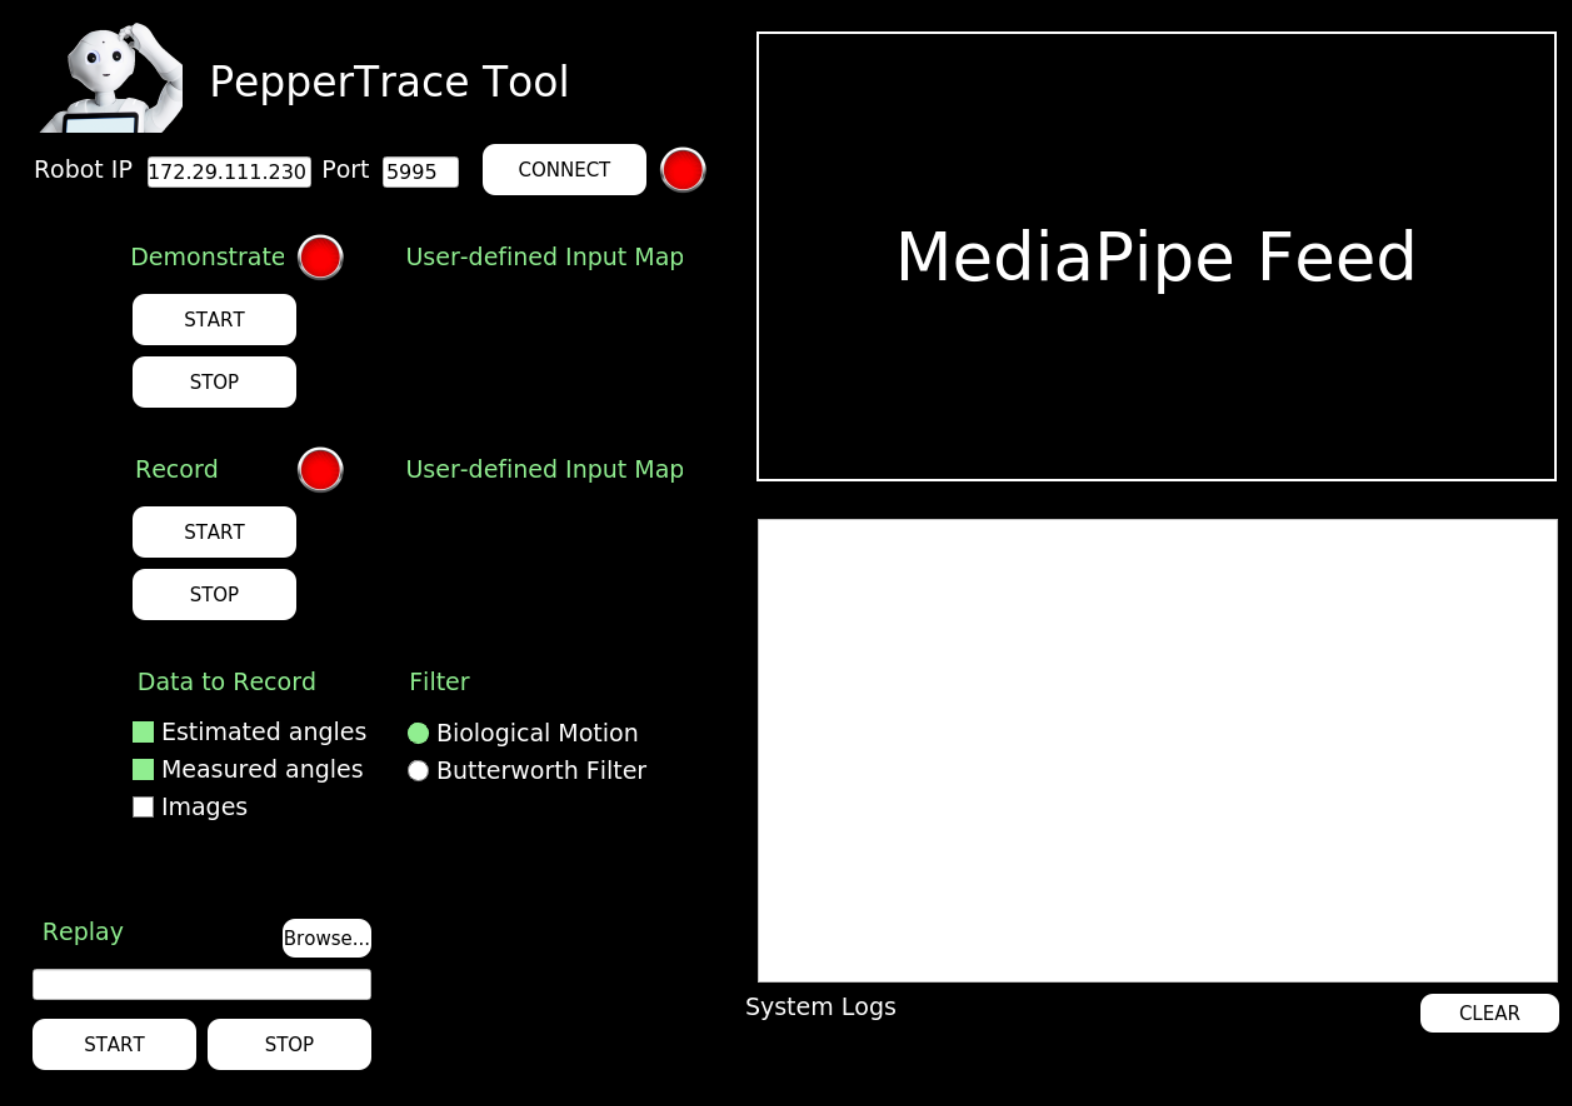
\includegraphics[width=\linewidth]{figures/peppertrace_gui.png}
    \caption{Graphical User Interface for the PepperTrace Programming by Demonstration Tool}
    \label{fig:gui}
\end{figure}
    
\newpage

\subsection*{(Optional) Configuration}
The \texttt{programming\_by\_demonstration} software package consists of three components, \texttt{skeletal\_model}, \texttt{demonstration\_recorder} and \texttt{demonstration\_gui}, each with configuration files in their \texttt{/config} folders. 

\begin{description}
    
    \item[Configure skeletal model:] Besides the camera intrinsics there are other configuration options in the config file of the \texttt{skeletal\_model} component, however it is not necessary to change them. 
        
    \item[Configure demonstration recorder: ] You can check and  configure where data recordings are stored in the configuration file of the \texttt{demonstration\_recorder} component through the \texttt{data\_dir} (base directory) and \texttt{demo\_name} (demo directory) parameters. It is not necessary to change the parameters.

    \item[Configure demonstration gui: ] You can configure some parameters for the GUI in the configuration file of the \texttt{demonstration\_gui} component. This is not necessary. 
       
    
\end{description}



\newpage

\section*{Main Features}

The PepperTrace GUI contains the following features for connecting to the robot, performing, recording and replaying demonstrations while logging imporant information for the user. 

\begin{description}
	\item[Connect: ] Enter the IP address and port of the Pepper robot and click the CONNECT button. This should connect the GUI to the Pepper robot and enable its controllers. Pressing the button again will stop the controllers and disconnect the robot.
    \item[Demonstrate: ] Press START under Demonstrate to enable demonstration. If a human is present in front of the camera, the software will capture its upper body movements and retarget them to Pepper in real time. Pressing STOP will stop this process.
	\item[Record: ] Press START under Record to record a demonstration. Check the boxes corresponding to the data that should be recorded during the demonstration. Demonstrate needs to be enabled for this to work. This will save the specified data to .bag files. 
	\item[Replay: ] Enter the path to a .bag file for replaying data and reproducing movement demonstrated in a previous recording session. Alternatively, click the Browse button and select the .bag file from the file dialog that appears. Click START to replay the bag file. The process will stop automatically when there is no more data to publish, unless you press STOP to before that. 
	\item[Logging: ] System logs (Infos, Warnings, Errors) are displayed to the System Logs box in the GUI. The skeletal model feed is displayed in the GUI when Demonstrate is on and the upper body joints of a human are detected in front of the camera. 
\end{description}

These features are illustrated in the behavioural graph in \cref{fig:behavioural}.

\begin{figure}[H]
    \centering
    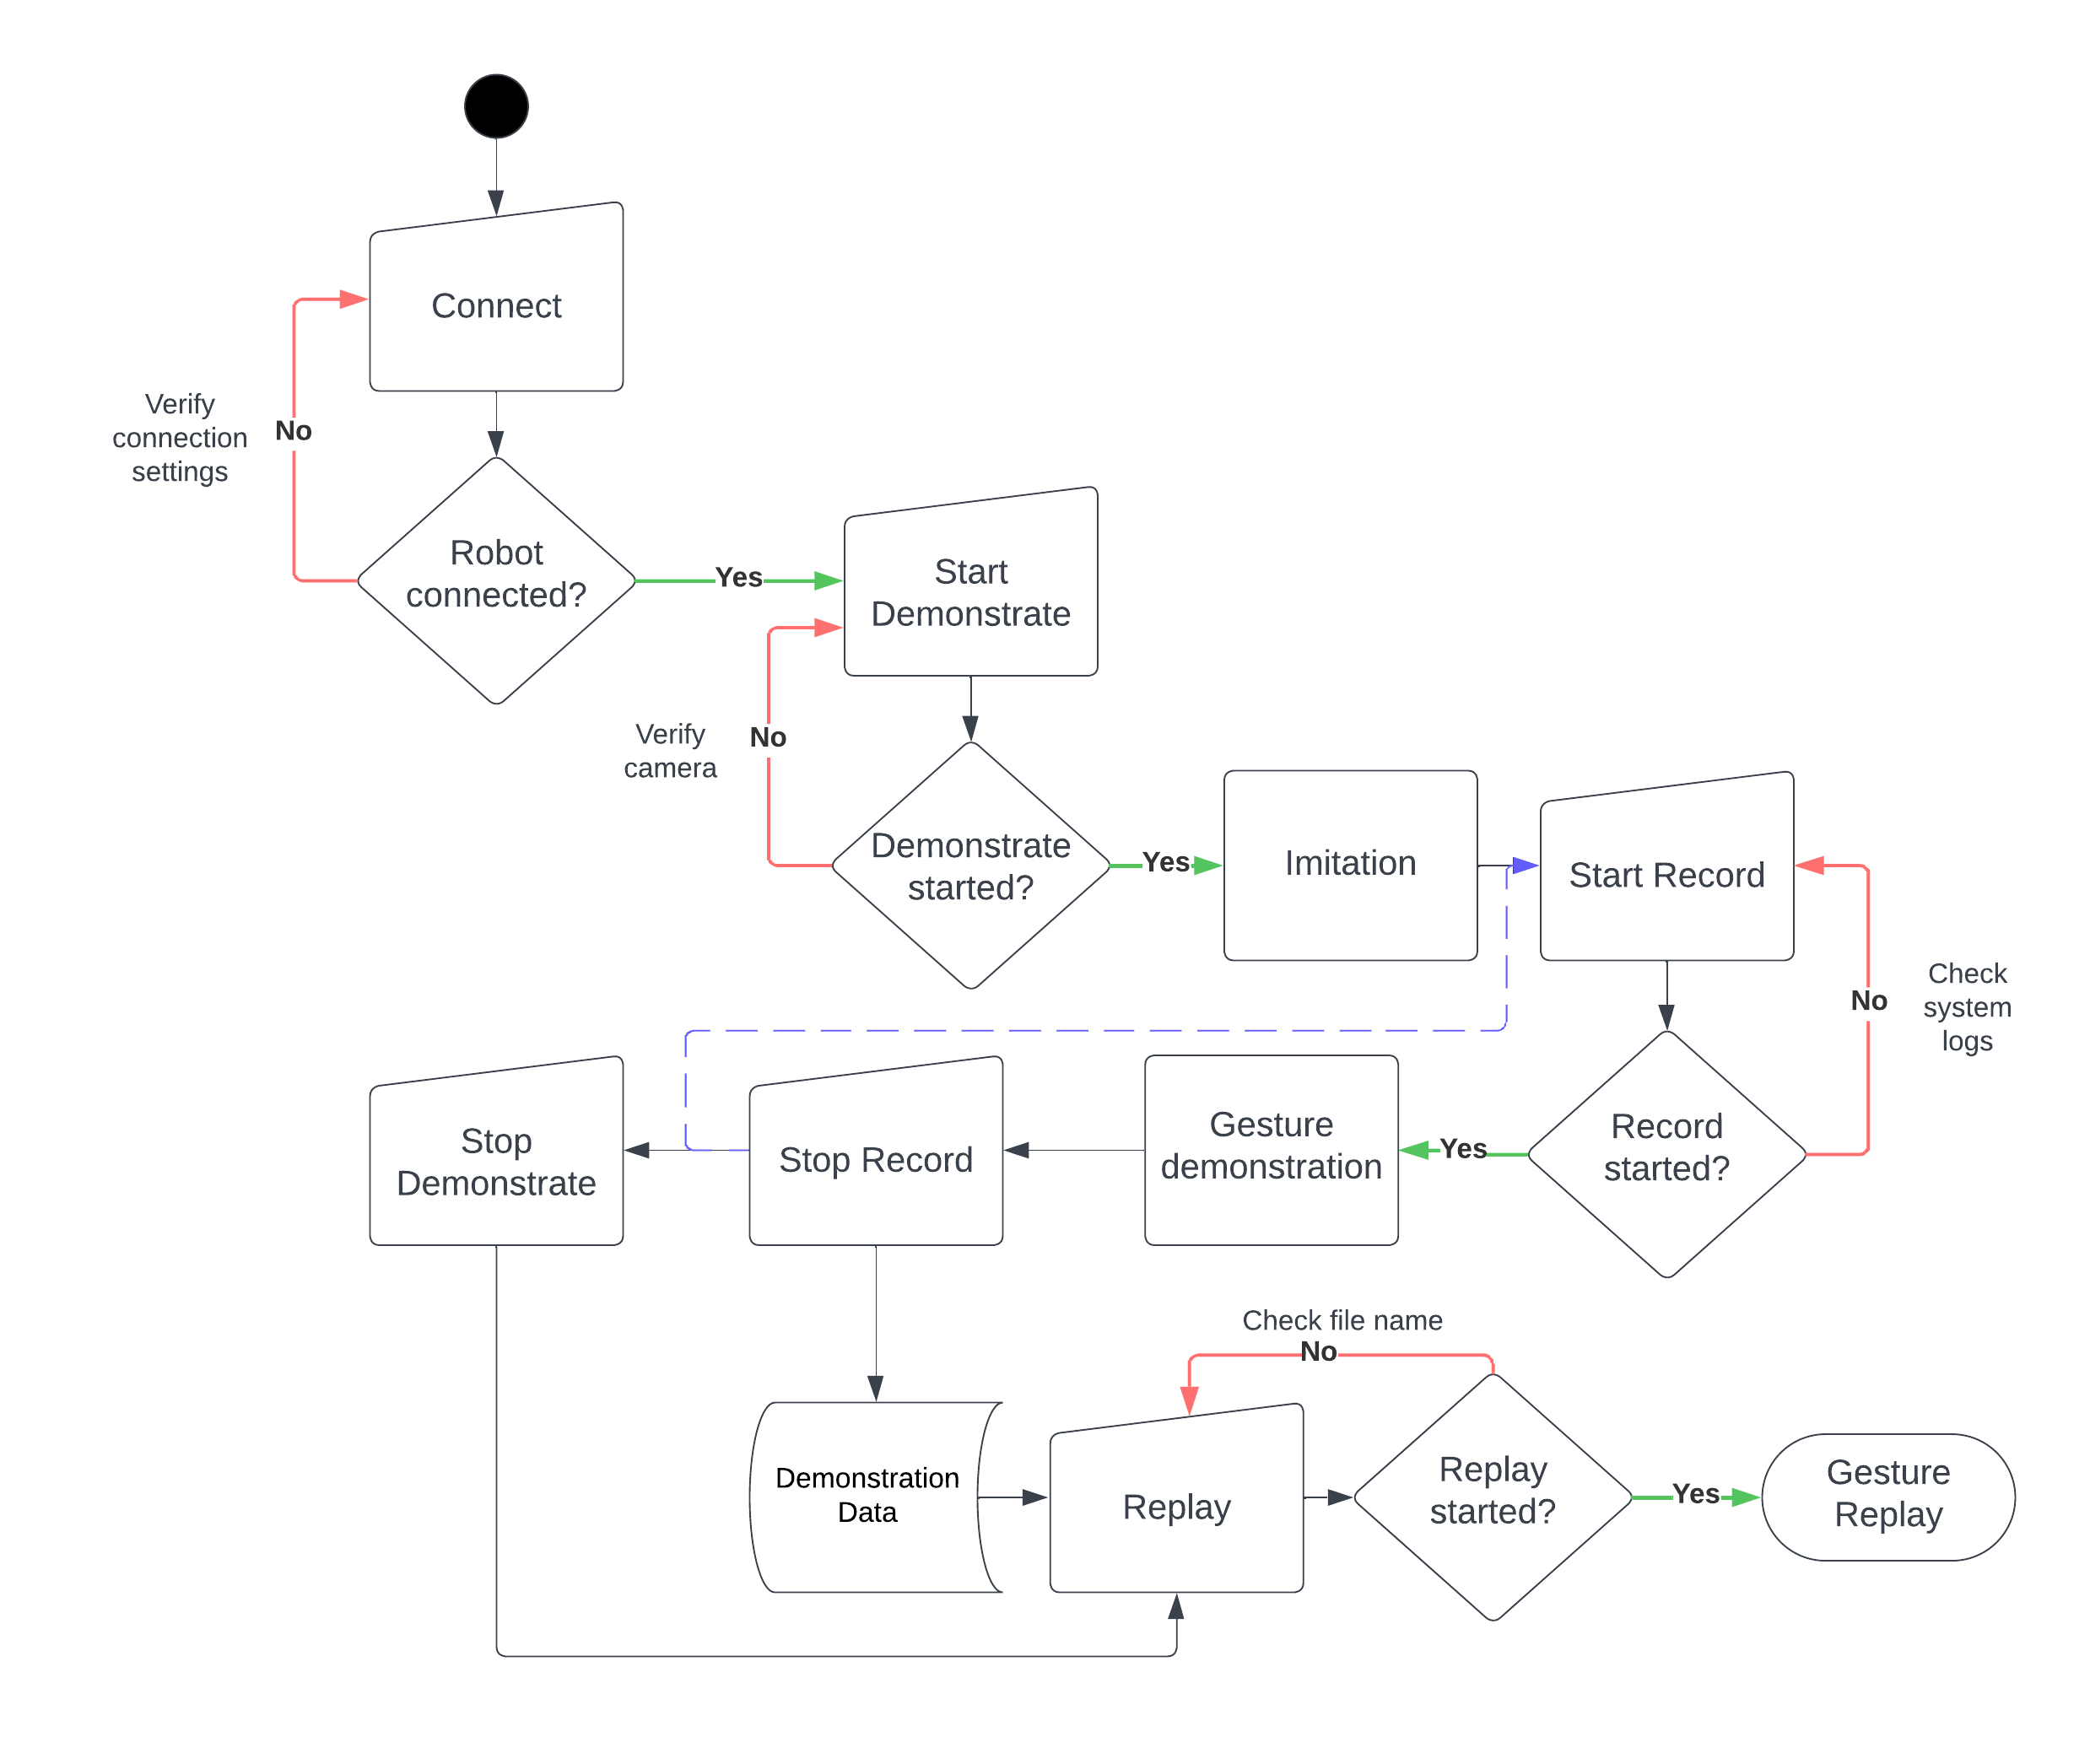
\includegraphics[width=\linewidth]{figures/BehaviouralGraph.png}
    \caption{Behavioural graph of the PbD module: The user-centered graph shows an example procedure for demonstrating, recording and replaying. Rectangular boxes represent observable processes, diamond-shaped boxes stand for checks, non-rectangular boxes represent user action. ``Gesture Replay" is the termination element. The blue line indicates the available option of recording multiple demonstrations in one session.}
    \label{fig:behavioural}
\end{figure}

\newpage

\section*{Guidelines for Reporting Issues} \label{sec:report}
%===============================================================
To report an issue or request a feature, please follow these steps:

\begin{description}
    \item[Step 1:] Go to the \href{https://github.com/danielcortezbarros/peppertrace}{Github repository} and go to ``Issues".

    \item[Step 2:] Check if your issue exists, otherwise open a new issue by clicking ``New issue".

    \item[Step 3:] Add a label to the issue:
    \begin{description}
        \item[bug:] For reporting something that is not working.
        \item[new\_feature:] For requesting a new feature.
        \item[docs:] For requesting further documentation.
        \item[question:] For general remarks.
    \end{description}

    \item[Step 4:] Please give a descriptive title and report the issue as clearly and with as much detail as possible, including code sections if applicable.

    \item[Step 5:] Follow and monitor the issue, as the developers may have follow-ups.
\end{description}



\newpage
\section*{Document History}
%================================================================
\addcontentsline{toc}{section}{Document History}
\label{document_history}

\begin{description}

\item [Version 1.0]~\\
First draft. \\
Daniel Barros. \\                                   
14 December 2024.                                                    
\item [Version 1.1]~\\
Formatting fixes.  \\
Daniel Barros. \\                                    
16 December 2024.   
\item [Version 1.2]~\\
Fixed formatting issues.  \\
Renumbered D5.5.1.L to D5.5.1.2  Programming by Demonstration.\\
Added Appendix I: User Manual --- PepperTrace Programming by Demonstration Tool.\\
David Vernon. \\                                   
6 January 2025.   
\item [Version 1.3]~\\
Fixed formatting issues.  \\
Changed \texttt{programming\_from\_demonstration}  to \texttt{programming\_by\_demonstration} throughout.\\
David Vernon. \\                                   
31 January 2025.   

\end{description}

\end{document}

